% !TEX TS-program = xelatexmk

\documentclass[12pt]{myNotes}

%%%%%%%%%%%%%%%%%%%%%%%%%%%%%%%%%%%%%%%%%%%%%%%%%%%%%%%%%%%%%%%%%%%%%%%%%%%
\usepackage[english]{babel}
\hyphenation{TOPPView}
\hyphenation{KNIME}
\hyphenation{OpenMS}

%%%%%%%%%%%%%%%%%%%%%%%%%%%%%%%%%%%%%%%%%%%%%%%%%%%%%%%%%%%%%%%%%%%%%%%%%%%
% FONT SELECTION -> WE NOW USE UBUNTU FONT AND XETEX FOR A MORE PROFESSIONAL
% LOOK.
% UBUNTU FONT CAN BE DOWNLOADED FROM HERE: http://font.ubuntu.com
%
\usepackage{fontspec}
\setmainfont[Ligatures = TeX]{Ubuntu-R.ttf}
\setmonofont[Ligatures = TeX]{Ubuntu-M.ttf}

% math fonts
%\usepackage[math-style=TeX]{unicode-math}
%\setmathfont{Cambria Math}


%%%%%%%%%%%%%%%%%%%%%%%%%%%%%%%%%%%%%%%%%%%%%%%%%%%%%%%%%%%%%%%%%%%%%%%%%%%
\usepackage{amsmath,amssymb,amscd,bm,dsfont,wasysym}
\usepackage{graphicx}
\usepackage[xetex,
      colorlinks=false,
      urlcolor=black,       % \href{...}{...} external (URL)
      filecolor=black,     % \href{...} local file
      linkcolor=black,       % \ref{...} and \pageref{...}
      citecolor=black,
      pdftitle={OpenMS Tutorial Handouts},
      pdfauthor={Johannes Veit},
      pdfsubject={},
      pdfkeywords={},
      pagebackref,
      pdfpagemode=none,
      bookmarksopen=true]{hyperref}

%%%%%%%%%%%%%%%%%%%%%%%%%%%%%%%%%%%%%%%%%%%%%%%%%%%%%%%%%%%%%%%%%%%%%%%%%%%

\newfontfamily{\menlo}{Menlo-Regular.ttf}

\usepackage{listings}
\usepackage{color}
\usepackage{textcomp}
\definecolor{listinggray}{gray}{0.9}
\definecolor{lbcolor}{rgb}{0.9,0.9,0.9}
\lstset{
    backgroundcolor=\color{lbcolor},
    tabsize=4,
    rulecolor=,
    language=python,
    basicstyle=\menlo\scriptsize,
    upquote=true,
    aboveskip={1.5\baselineskip},
    columns=fixed,
    showstringspaces=false,
    extendedchars=true,
    breaklines=true,
    prebreak = \raisebox{0ex}[0ex][0ex]{\ensuremath{\hookleftarrow}},
    frame=single,
    showtabs=false,
    showspaces=false,
    showstringspaces=false,
    identifierstyle=\menlo,
    keywordstyle=\color[rgb]{0,0,1},
    commentstyle=\color[rgb]{0.133,0.545,0.133},
    stringstyle=\color[rgb]{0.627,0.126,0.941},
}

%%%%%%%%%%%%%%%%%%%%%%%%%%%%%%%%%%%%%%%%%%%%%%%%%%%%%%%%%%%%%%%%%%%%%%%%%%%
% only use those two in combination
\usepackage[textsize=scriptsize]{todonotes}
%\usepackage[firstpage]{draftwatermark}
%\SetWatermarkScale{4}

%%%%%%%%%%%%%%%%%%%%%%%%%%%%%%%%%%%%%%%%%%%%%%%%%%%%%%%%%%%%%%%%%%%%%%%%%%%
% better key and menu tips
\usepackage{menukeys}
\renewmenumacro{\directory}[/]{pathswithfolder}

%%%%%%%%%%%%%%%%%%%%%%%%%%%%%%%%%%%%%%%%%%%%%%%%%%%%%%%%%%%%%%%%%%%%%%%%%%%
% easy referencing
\usepackage[noabbrev,capitalise]{cleveref}

%%%%%%%%%%%%%%%%%%%%%%%%%%%%%%%%%%%%%%%%%%%%%%%%%%%%%%%%%%%%%%%%%%%%%%%%%%%
% subfigures
\usepackage{subcaption}

%%%%%%%%%%%%%%%%%%%%%%%%%%%%%%%%%%%%%%%%%%%%%%%%%%%%%%%%%%%%%%%%%%%%%%%%%%%
% boxes with notes
%%%%%%%%%%%%%%%%%%%%%%%%%%%%%%%%%%%%%%%%%%%%%%%%%%%%%%%%%%%%%%%%%%%%%%%%%%%
\usepackage{tikz}
\usetikzlibrary[shadows]
\usepackage[framemethod=TikZ]{mdframed}
\usetikzlibrary{calc}

\global\mdfdefinestyle{notedefault}{topline=false,bottomline=false,rightline=false,leftmargin=1cm}
\newcommand{\note}[1]{ \begin{mdframed}[style=notedefault] \textbf{Note:}~#1 \end{mdframed} }

%%%%%%%%%%%%%%%%%%%%%%%%%%%%%%%%%%%%%%%%%%%%%%%%%%%%%%%%%%%%%%%%%%%%%%%%%%%
\newmdenv[
  leftmargin=0pt,
  rightmargin=20pt,
  innertopmargin=30pt,
  innerbottommargin=10pt,
  innerleftmargin=45pt,
  middlelinewidth=0pt,
  linecolor=black,
  topline=false,
  bottomline=false,
  rightline=false,
  font=\normalfont\normalsize,
  frametitlefont=\normalfont\normalsize\bfseries,
  frametitleaboveskip=1em,
  singleextra={
    \node[inner sep=0pt,anchor=north west,xshift=10pt,yshift=-30pt] at (P-|O) {
\includegraphics[width=1.3cm]{graphics/assets/question23}};
    \node[inner sep=0pt,anchor=north west,yshift=-.8\baselineskip,font=\bfseries,xshift=10pt] at (P-|O) {Question};
  },
  firstextra={
    \node[inner sep=0pt,anchor=north west,xshift=10pt,yshift=-30pt] at (P-|O) {
\includegraphics[width=1.3cm]{graphics/assets/question23}};
    \node[inner sep=0pt,anchor=north west,yshift=-.8\baselineskip,font=\bfseries,xshift=10pt] at (P-|O) {Question};
  }
]{question}

%%%%%%%%%%%%%%%%%%%%%%%%%%%%%%%%%%%%%%%%%%%%%%%%%%%%%%%%%%%%%%%%%%%%%%%%%%%
\newmdenv[
  leftmargin=0pt,
  rightmargin=20pt,
  innertopmargin=30pt,
  innerbottommargin=10pt,
  innerleftmargin=45pt,
  middlelinewidth=0pt,
  linecolor=black,
  topline=false,
  bottomline=false,
  rightline=false,
  font=\normalfont\normalsize,
  frametitlefont=\normalfont\normalsize\bfseries,
  frametitleaboveskip=1em,
  singleextra={
    \node[inner sep=0pt,anchor=north west,xshift=10pt,yshift=-30pt] at (P-|O) {
\includegraphics[width=1.3cm]{graphics/assets/check30}};
    \node[inner sep=0pt,anchor=north west,yshift=-.8\baselineskip,font=\bfseries,xshift=10pt] at (P-|O) {Task};
  },
  firstextra={
    \node[inner sep=0pt,anchor=north west,xshift=10pt,yshift=-30pt] at (P-|O) {
\includegraphics[width=1.3cm]{graphics/assets/check30}};
    \node[inner sep=0pt,anchor=north west,yshift=-.8\baselineskip,font=\bfseries,xshift=10pt] at (P-|O) {Task};
  }
]{task}

%%%%%%%%%%%%%%%%%%%%%%%%%%%%%%%%%%%%%%%%%%%%%%%%%%%%%%%%%%%%%%%%%%%%%%%%%%%
\newcommand{\KNIMENODE}[1]{\texttt{#1}}
\newcommand{\OPENMSTOOL}[1]{\texttt{#1}}

\begin{document}
%%%%%%%%%%%%%%%%%%%%%%%%%%%%%%%%%%%%%%%%%%%%%%%%%%%%%%%%%%%%%%%%%%%%%%%%%%%

\firstpages

%%%%%%%%%%%%%%%%%%%%%%%%%%%%%%%%%%%%%%%%%%%%%%%%%%%%%%%%%%%%%%%%%%%%%%%%%%%

\setcounter{equation}{0}
\section{General remarks}
\label{General remarks}

\begin{itemize}
\item This handout will guide you through an introductory tutorial for the OpenMS/TOPP software package~\cite{OpenMS}.
\item OpenMS~\cite{Sturm2008} is a versatile open-source library for mass spectrometry data analysis. Based on this library, we offer a collection
      of command-line tools ready to be used by end users. These so-called TOPP tools (short for ``The OpenMS Proteomics Pipeline'')~\cite{Kohlbacher2007} can be understood as
      small building blocks of arbitrary complex data analysis workflows.
\item In order to facilitate workflow construction, OpenMS was integrated into KNIME~\cite{KNIME}, the Konstanz
			Information Miner, an open-source integration platform providing a powerful and flexible workflow system
			combined with advanced data analytics, visualization, and report capabilities. Raw MS data as well as the
			results of data processing using TOPP can be visualized using TOPPView~\cite{Sturm2009}.
\item In this hands-on tutorial session, you will become familiar with some of the basic functionalities of OpenMS/TOPP, TOPPView, and KNIME
      and learn how to use a selection of TOPP tools used in the tutorial workflows.
\item All data referenced in this tutorial can be found in the \directory{Example\_Data} folder that came with this tutorial.
\end{itemize}

%%%%%%%%%%%%%%%%%%%%%%%%%%%%%%%%%%%%%%%%%%%%%%%%%%%%%%%%%%%%%%%%%%%%%%%%%%%
%\newpage
%!TEX root = handout.tex

\setcounter{equation}{0}

%%%%%%%%%%%%%%%%%%%%%%%%%%%%%%%%%%%%%%%%%%%%%%%%%%%%%%%%%%%%%%%%%%%%%%%%%%%%%%%%
\section{Getting started}

\subsection{Data conversion}
\label{Data_Conversion}

Each MS instrument vendor has one or more formats for storing the acquired data. Converting these data into an open format (preferably mzML) is the very first step when you want to work with open-source mass spectrometry software. A freely available conversion tool is ProteoWizard. The OpenMS installation package for Windows automatically installs ProteoWizard, so you do not need to download and install it separately.

Please note that due to restrictions from the instrument vendors, file format conversion for most formats is only possible on Windows systems, so exporting from the acquisition PC connected to the instrument is usually the most convenient option.
All files used in this tutorial have already been converted to mzML by us, so you do not need to do it yourself.

%%%%%%%%%%%%%%%%%%%%%%%%%%%%%%%%%%%%%%%%%%%%%%%%%%%%%%%%%%%%%%%%%%%%%%%%%%%%%%%%

\subsection{Data visualization using \OPENMSTOOL{TOPPView}}
\label{Data_Visualization}

Visualizing the data is the first step in quality control, an essential tool in understanding the data, and of course an essential step in pipeline development.
OpenMS provides a convenient viewer for some of the data: \OPENMSTOOL{TOPPView}.

\begin{figure}
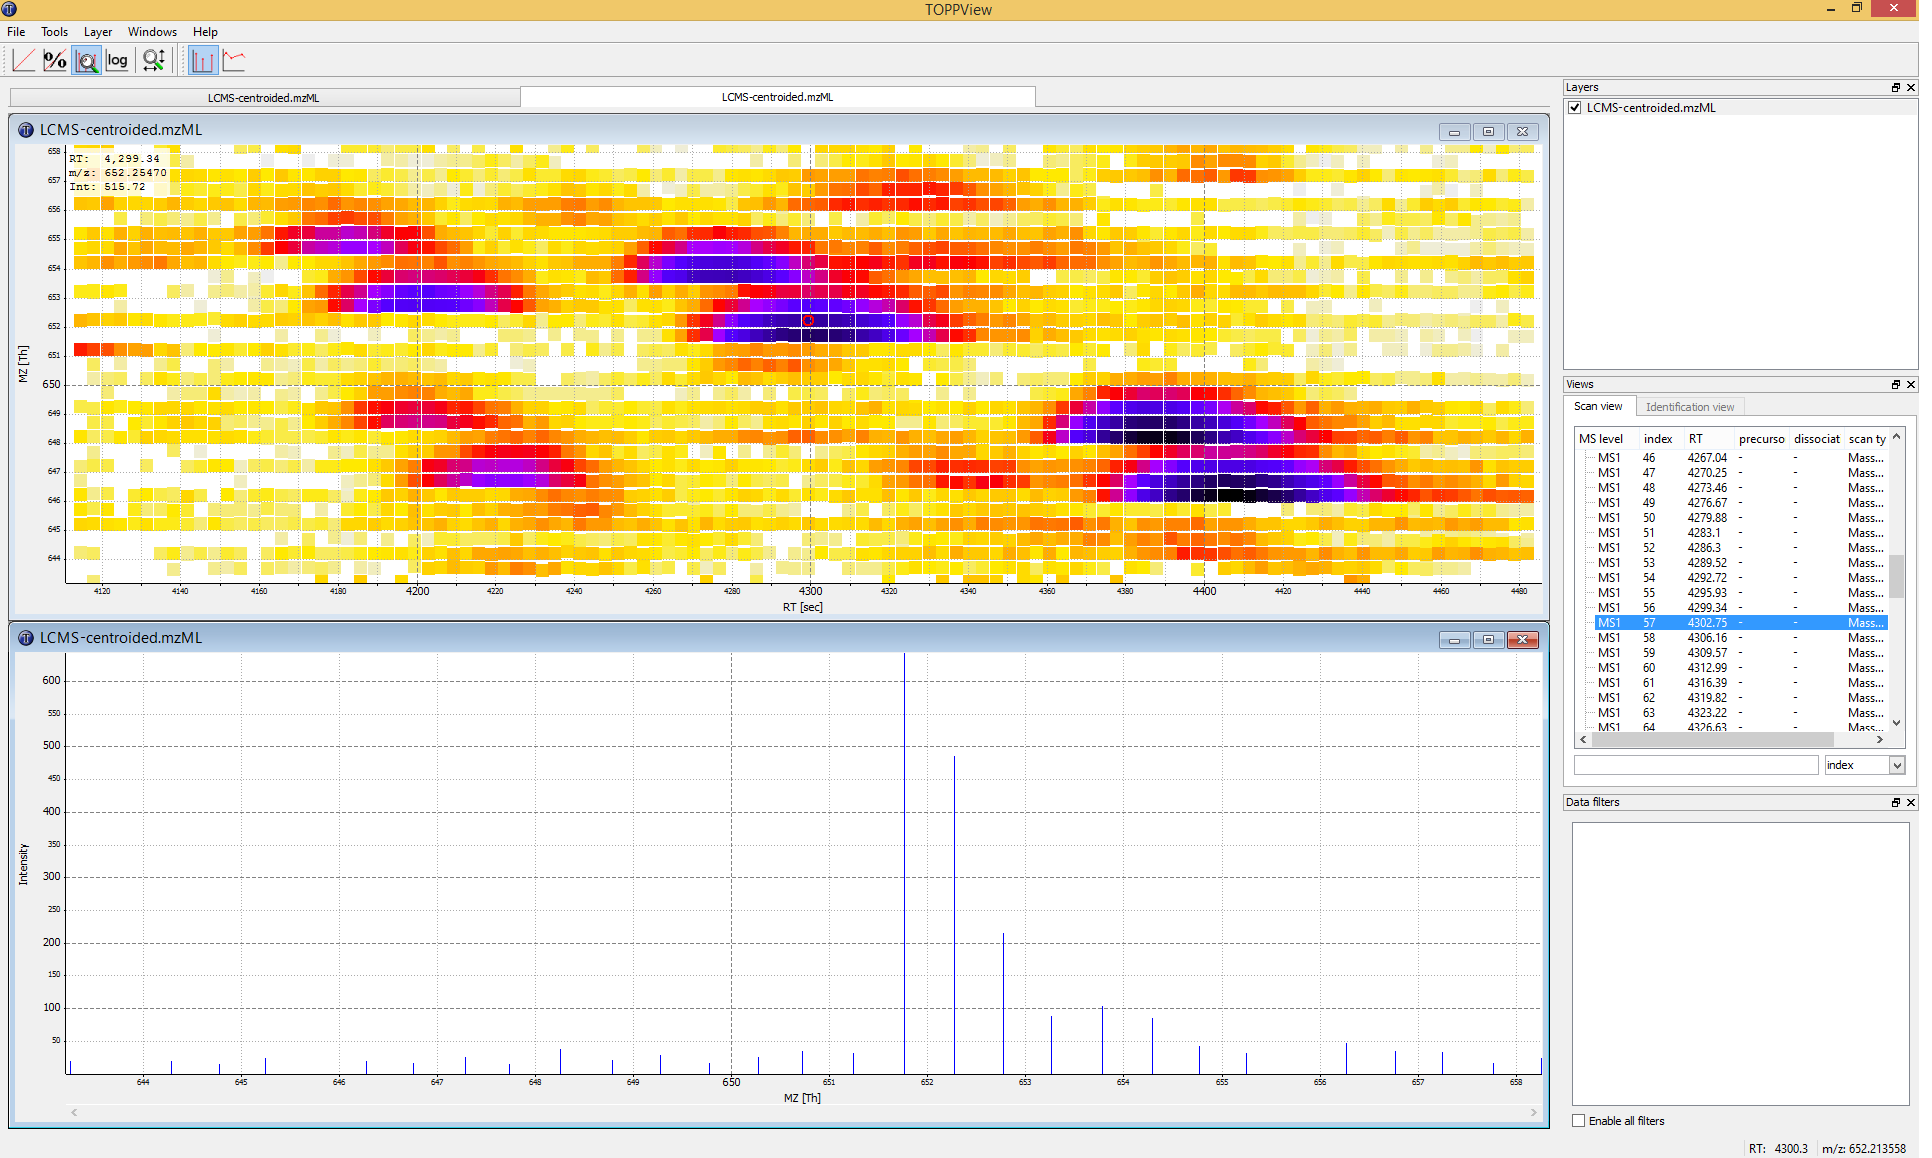
\includegraphics[width=\textwidth]{graphics/introduction/TOPPView.png}
\caption{TOPPView, the graphical application for viewing mass spectra and analysis results. Top window shows a small region of a peak map. In this 2D representation of the measured spectra, signals of eluting peptides are colored according to the raw peak intensities. The lower windows displays an extracted spectrum (=scan) from the peak map. On the right side, the list of spectra can be browsed.}
\label{fig:toppview}
\end{figure}

We will guide you through some of the basic features of \OPENMSTOOL{TOPPView}. Please familiarize yourself with the key controls and visualization methods.
We will make use of these later throughout the tutorial. Let's start with a first look at one of the files of our tutorial data set:

\begin{itemize}
\item Start \OPENMSTOOL{TOPPView} (see Start-Menu or Applications on MacOS)
\item Go to \menu{File > Open File}, navigate to the directory where you copied the contents of the USB stick to,
      and select
      \directory{Example\_Data / Introduction / datasets / small / velos005614.mzML}
      . This file contains a reduced LC-MS map (only a selected RT and m/z range
      was extracted using the TOPP tool \OPENMSTOOL{FileFilter}) of a label-free measurement of the human platelet proteome recorded on an Orbitrap velos.
      The other two mzML files contain technical replicates of this experiment.
      First, we want to obtain a global view on the whole LC-MS map - the default option \textit{Map view 2D} is the correct one and we can click the ok button. 
\item Play around.
\item Three basic modes allow you to interact with the displayed data: scrolling, zooming and measuring:
    \begin{itemize}
    \item Scroll mode
        \begin{itemize}
        \item Is activated by default (though each loaded spectra file is displayed zoomed out first, so you do not need to scroll).
        \item Allows you to browse your data by moving around in RT and m/z range.
        \item When zoomed in, to scroll the spectra map, click-drag on the current view.
        \item Arrow keys can be used to scroll the view as well.
        \end{itemize}
    \item Zoom mode
        \begin{itemize}
        \item Zooming into the data: either mark an area in the current view with your mouse while holding the left mouse
              button plus the \keys{\ctrl} key to zoom to this area
              or use your mouse wheel to zoom in and out.
        \item All previous zoom levels are stored in a zoom history. The zoom history can be traversed using
              \keys[,]{\ctrl,+} or \keys[,]{\ctrl,-} or the mouse wheel (scroll up and down).
        \item Pressing the Backspace key zooms out to show the full LC-MS map (and also resets the zoom history).
        \end{itemize}
    \item Measure mode
        \begin{itemize}
        \item It is activated using the \keys{\shift} key.
        \item Press the left mouse button down while a peak is selected and drag the mouse to
        			another peak to measure the distance between peaks.
        \item This mode is implemented in the 1D and 2D mode only.
        \end{itemize}
    \end{itemize}
\item Right click on your 2D map and select \menu{Switch to 3D view} and examine your
			data in 3D mode
\item Go back to the 2D view. In 2D mode, visualize your data in different normalization modes, use linear, percentage and log-view (icons on the upper left tool bar).
\note{On \textit{Apple OS X}, due to a bug in one of the external libraries used by OpenMS, you will see a small window of the 3D mode when switching to 2D. Close the 3D tab in order to get rid of it.}
\item In \OPENMSTOOL{TOPPView} you can also execute TOPP tools. Go to
			\menu{Tools > Apply tool (whole layer)} and choose a TOPP tool (e.g., FileInfo) and
			inspect the results.
\end{itemize}

%%%%%%%%%%%%%%%%%%%%%%%%%%%%%%%%%%%%%%%%%%%%%%%%%%%%%%%%%%%%%%%%%%%%%%%%%%%%%%%%

\subsection{Introduction to KNIME / OpenMS}
\label{KNIME_Intro}

Using OpenMS in combination with KNIME you can create, edit, open, save, and run workflows
combining TOPP tools with the powerful data analysis capabilities of KNIME. Workflows can
be created conveniently in a graphical user interface. The parameters of all involved
tools can be edited within the application and are also saved as part of the workflow.
Furthermore, KNIME interactively performs validity checks during the workflow editing
process, in order to make it more difficult to create an invalid workflow.

Throughout most of the parts of this tutorial you will use KNIME to create and
execute workflows. This first step is to make yourself familiar with KNIME.

% 
% This description is based on KNIME 1.12.0
%

\subsubsection{Install OpenMS using KNIME}

Before we can start with the tutorial we need to install all the required extensions for KNIME.

First, we install some additional extensions that are required by our OpenMS nodes or used in the Tutorials e.g. for visualization.
\begin{enumerate}
\item Click on \menu{Help > Install New Software...}
\item From the \menu{Work with:} drop down list select \menu{http://update.knime.org/analytics-platform/2.12}
\item Now select the following plugins from the \textit{KNIME \& Extensions} category
    \begin{itemize}
    \item KNIME Base Chemistry Types \& Nodes
    \item KNIME Chemistry Add-Ons
    \item KNIME File Handling Nodes
    \item KNIME Interactive R Statistics Integration
    \item KNIME Math Expression (JEP)
    \item KNIME Report Designer
    \item KNIME SVG Support
    \item KNIME XLS Support
    \item KNIME XML-Processing
    \end{itemize}
%\item And the following plugin from the \textit{Marvin Chemistry Extensions (donated by Infocom \& Chemaxon)} category
%    \begin{itemize}
%    \item ChemAxon/Infocom Marvin Extensions Feature
%    \end{itemize}
\item From the \menu{Work with:} drop down list select \\\menu{http://tech.knime.org/update/community-contributions/trusted/2.12}
\item Now select the following plugin from the \textit{KNIME Community Contributions - Cheminformatics} category 	
    \begin{itemize}
    \item     RDKit KNIME integration
    \end{itemize}	
\item Follow the instructions and after a restart of KNIME the dependencies will be installed.
\end{enumerate}

You are now ready to install the OpenMS nodes.

\begin{enumerate}
\item Open KNIME.
\item Click on \menu{Help > Install New Software...}
  
% Use this part if you base the tutorial on the nightly contributions (not recommended - more of a emergency measure)
  %\item \label{it:add_site} In the now open dialog choose \menu{Add...} (in the upper right corner of the dialog) to define a new update site. In the opening dialog enter the following details. \\
  %\textit{Name:} \texttt{Trunk Community Contributions} \\
  %\textit{Location:} \texttt{http://tech.knime.org/update/community-contributions/trunk/}
  %\item \label{it:select_site} After pressing \keys{OK} KNIME will show you all the contents of the added Update Site.

% Use this part if you base the tutorial on the last stable release (recommended)
  \item From the \menu{Work with:} drop down list select the \\ \menu{http://tech.knime.org/update/community-contributions/trusted/2.12}
\item Select the \textbf{OpenMS} nodes in the category: \\ "KNIME Community Contributions - Bioinformatics \& NGS" and click \keys{Next}.
\item Follow the instructions and after a restart of KNIME the OpenMS nodes will be available under “Community Nodes”.
\end{enumerate}

% Use this part if you base the tutorial on a pre-release of OpenMS X.X.X
 %\note{
 %For this tutorial we use a pre-release version of OpenMS X.X.X
 %While not being a full release, it was nevertheless intensively tested to ensure its functionality for this tutorial.
 %For regular use we recommend using the latest stable OpenMS release.
 %Please note that some of the workflows shown here require OpenMS X.X and therefore will not work with OpenMS Y.Y downloaded from the stable update site.
 %}

\subsubsection{KNIME concepts}

A \textbf{workflow} is a sequence of computational steps applied to a single or multiple input data sets to process and analyze the data.
In KNIME such workflows are implemented graphically by combining so-called \textbf{nodes}.
A node represents a single analysis step in a workflow.
Nodes have input and output \textbf{ports} where the data enters the node or the results are provided for other nodes after processing, respectively.
KNIME distinguishes between different port types, representing different types of data.
The most common representation of data in KNIME are tables (similar to an excel sheet).
Ports that accept tables are marked with a small triangle.
For OpenMS we use a different port type, so called \textbf{file ports}, representing complete files.
Those ports are marked by a small grey box.
Dark grey boxes represent mandatory inputs and light grey boxes optional inputs.

A typical OpenMS workflow in KNIME can be divided in two conceptually different parts:
\begin{itemize}
\item
Nodes for signal and data processing, filtering and data reduction. Here, files are passed between nodes. Execution times of the individual steps are longer as the main computational steps are performed. 
\item
Downstream statistical analysis and visualization. Here, tables are passed between nodes.
\end{itemize}

Between file based processing and table based analysis a conversion node typically performs the conversion from OpenMS results into KNIME tables.

Nodes can have three different states, indicated by the small traffic light below the node.

\begin{itemize}
\item
Inactive, failed, and not yet fully configured nodes are marked red.
\item
Configured but not yet executed nodes are marked yellow.
\item
Successfully executed nodes are marked green.
\end{itemize}

If the node execution failed the node will switch to the red state.

Most nodes will be configured as soon as all input ports are connected.
For some nodes additional parameters have to be provided that cannot be either guessed from the data or filled with sensible defaults.
In this case, of if you want to customize the default configuration, you can open the configuration dialog of a node with a double-click on the node.
For OpenMS you will see a configuration dialog like the one shown in \cref{fig:knime_configure}.
\note{OpenMS distinguishes between normal parameters and advanced parameters.
Advanced parameters are by default hidden from the users since they should only rarely be customized.
In case you want to have a look at the parameters or need to customize them in one of the tutorials you can show them by clicking on the checkbox  \menu{Show advanced parameter} in the lower part of the dialog.}
The dialog shows the individual parameters, their current value and type, and, in the lower part of the dialog, the documentation for the currently selected parameter.

\begin{figure}
\centering
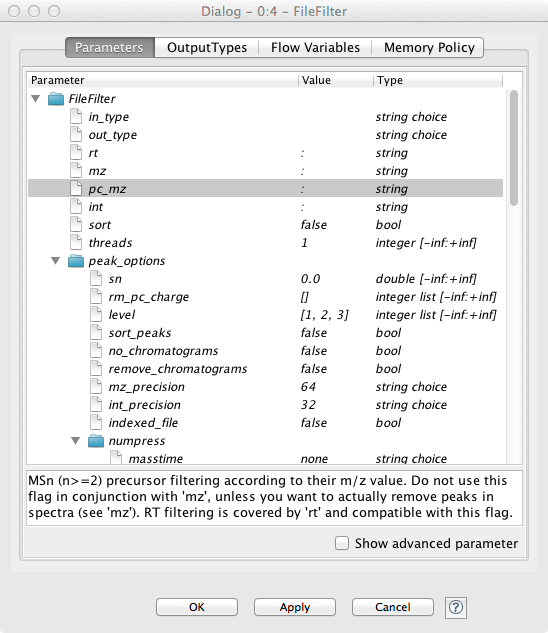
\includegraphics[width=0.5\textwidth]{graphics/knime_setup/knime_configure_dialog}
\caption{Node configuration dialog of an OpenMS node.}
\label{fig:knime_configure}
\end{figure}

\subsubsection{Overview of the graphical user interface}

\begin{figure}
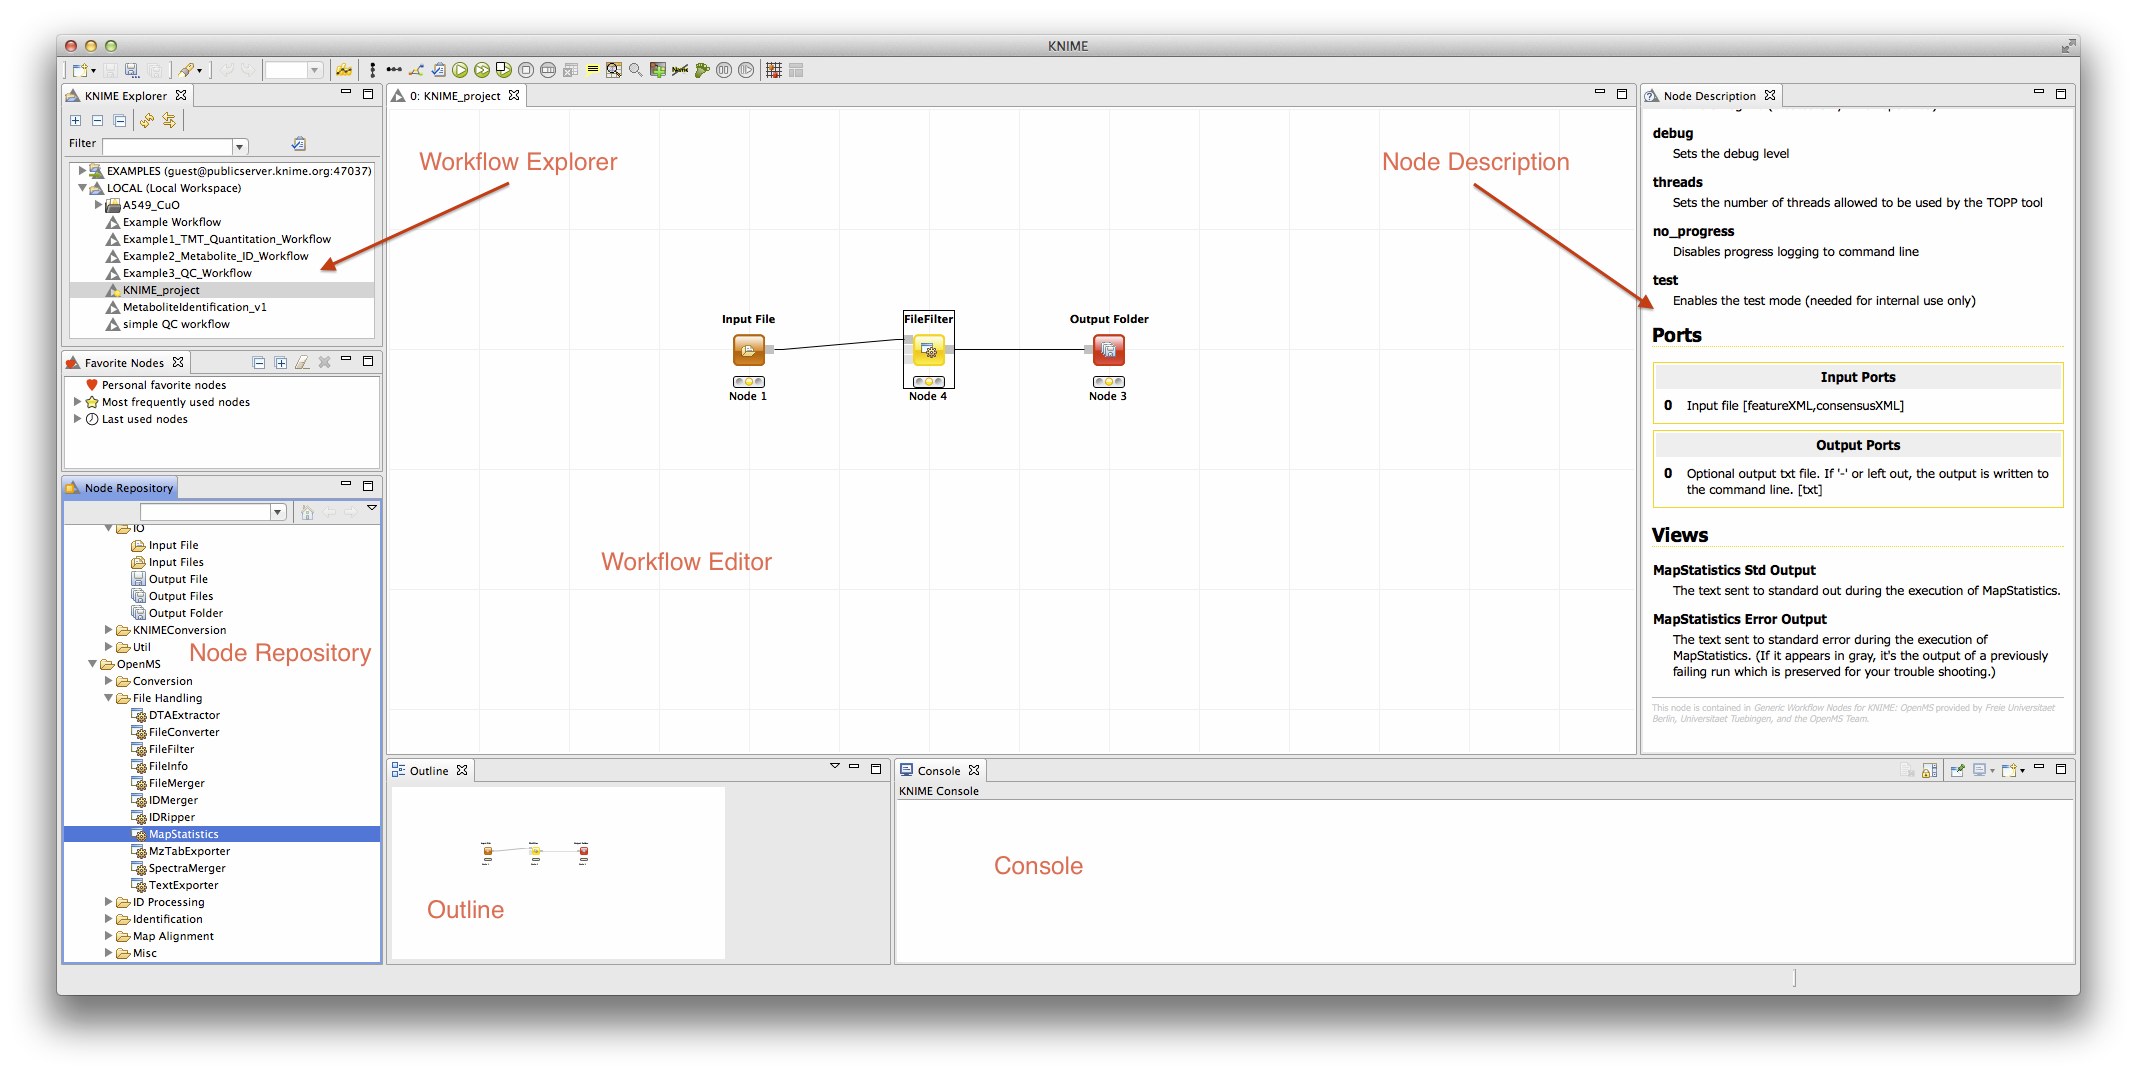
\includegraphics[width=\textwidth]{graphics/knime_setup/knime_workbench_marked}
\caption{The KNIME workbench.}
\label{fig:knime_workbench}
\end{figure}

The graphical user interface (GUI) of KNIME consists of different components or so called panels that are shown in \cref{fig:knime_workbench}.
We will shortly introduce the individual panels and their purpose below.

\begin{description}
\item[Workflow Editor]
The workflow editor is the central part of the KNIME GUI.
Here you assemble the workflow by adding nodes from the Node Repository via "drag \& drop".
Nodes can be connected by clicking on the output port of one node and releasing the mouse at the desired input port of the next node.

\item[Workflow Explorer]
Shows a list of available workflows (also called workflow projects).
You can open a workflow by double clicking it.
A new workflow can be created with a right-click in the Workflow Explorer followed by selecting \menu{New KNIME Workflow...}.

\item[Node Repository]
Shows all nodes that are available in your KNIME installation.
Every plugin you install will provide new nodes that can be found here.
The OpenMS nodes can be found in \menu{Community Nodes > OpenMS}.
Nodes for managing files (e.g., Input Files or Output Folders) can be found in \menu{Community Nodes > GenericKnimeNodes}.
You can search the node repository by typing the node name into the small text box in the upper part of the node repository.

\item[Outline]
The Outline panel contains a small overview of the complete workflow. While of limited use when working on a small workflow, this feature is very helpful as soon as the workflows get bigger.

\item[Console]
In the console panel warning and error messages are shown.
This panel will provide helpful information if one of the nodes failed or shows an warnings sign.

\item[Node Description]
As soon as a node is selected, the Node Description window will show the documentation of the node including documentation for all its parameters.
For OpenMS nodes you will also find a link to the tool page in the online documentation.

\end{description}

\subsubsection{Creating workflows}
\label{sec:create_workflows}

Workflows can easily be created by a right click in the Workflow Explorer followed by clicking on \menu{New KNIME Workflow...}.

\subsubsection{Sharing workflows}
\label{sec:sharing_workflows}

To be able to share a workflow with others, KNIME supports the import and export of complete workflows.
To export a workflow, select it in the Workflow Explorer and select \menu{File > Export KNIME Workflow...}.
KNIME will export workflows as a zip file containing all the information on nodes, their connections, and their configuration.
Those zip files can again be imported by selecting \menu{File > Import KNIME Workflow...}.

\note{For your convenience we added all workflows discussed in this tutorial to the \directory{Workflows} folder.
If you want to check your own workflow by comparing it to the solution or got stuck, simply import the full workflow from the corresponding zip file.}

\subsubsection{Duplicating workflows}
\label{sec:duplicate-wf}

During the tutorial a lot of the workflows will be created based on the workflow from a previous task.
To keep the intermediate workflows we suggest you create copies of your workflows so you can see the progress.
To create a copy of your workflow follow the following steps

\begin{itemize}
\item
Right click on the workflow you want to create a copy of in the Workflow Explorer and select \menu{Copy}.
\item
Right click again somewhere on the workflow explorer and select \menu{Paste}.
\item
This will create a workflow with same name as the one you copied with a (2) appended.
\item
To distinguish them later on you can easily rename the workflows in the Workflow Explorer by right clicking on the workflow and selecting \menu{Rename}. \note{To rename a workflow it has to be closed.}
\end{itemize}

\subsubsection{A minimal workflow}
\label{Minimal_Workflow}

Let us now start with the creation of our very first, very simple workflow.
As a first step, we will gather some basic information about the data set before starting the
actual development of a data analysis workflow.

\begin{itemize}
\item
Create a new workflow.
\item Add an \KNIMENODE{Input File} node and an \KNIMENODE{Output Folder} node (to be found in \menu{Community Nodes > GenericKnimeNodes > IO} and a \KNIMENODE{FileInfo} node (to be found in the category \menu{Community Nodes > OpenMS > File Handling}) to the workflow.
\item Connect the \KNIMENODE{Input File} node to the \KNIMENODE{FileInfo} node, and the first output port of the \KNIMENODE{FileInfo} node to the \KNIMENODE{Output Folder} node.
\note{In case you are unsure about which node port to use, hovering the cursor over the port in question will display the port name and what kind of input it expects.}
The complete workflow is shown in \cref{fig:knime_minimal}.
FileInfo can produce two different kinds of output files.
\item All nodes are still marked red, since we are missing an actual input file.
Double-click the Input File node and select \menu{Browse}.
In the file system browser select \directory{Example\_Data / Introduction / datasets / tiny / velos005614.mzML} and click \menu{Open}.
Afterwards close the dialog by clicking \menu{Ok}.
\note{Make sure to use the ``tiny'' version this time, not ``small'', for the sake of faster workflow execution.}
\item The \KNIMENODE{Input File} node and the \KNIMENODE{FileInfo} node should now have switched to yellow, but the \KNIMENODE{Output Folder} node is still red.
Double-click on the \KNIMENODE{Output Folder} node and click on \menu{Browse} to select an output directory for the generated data.
\item Great! Your first workflow is now ready to be run. Press \keys{\shift + F7} to execute the complete workflow.
You can also right click on any node of your workflow and select \menu{Execute} from the context menu.
\item The traffic lights tell you about the current status of all nodes in your workflow.
Currently running tools show either a progress in percent or a moving blue bar, nodes waiting for data show the small word ``queued'', and successfully executed ones become green.
If something goes wrong (e.g., a tool crashes), the light will become red.
\item In order to inspect the results, you can just right-click the \KNIMENODE{Output Folder} node and select \menu{View: Open the output folder}.
You can then open the text file and inspect its contents.
You will find some basic information of the data contained in the mzML file, e.g., the total number of spectra and peaks, the RT and m/z range, and how many MS1 and MS2 spectra the file contains.
\end{itemize}

\begin{figure}
\centering
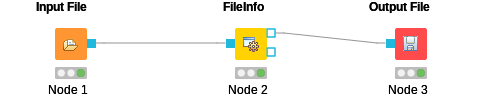
\includegraphics[width=0.59\textwidth]{graphics/knime_setup/Minimal_FileInfo}
\caption{A minimal workflow calling FileInfo on a single file.}
\label{fig:knime_minimal}
\end{figure}


Workflows are typically constructed to process a large number of files automatically.
As a simple example, consider you would like to gather this information for more than one file.
We will now modify the workflow to compute the same information on three different files and then write the output files to a folder.

\begin{itemize}
\item
We start from the previous workflow.
\item
First we need to replace our single input file with multiple files.
Therefore we add the \KNIMENODE{Input Files} node from the category \menu{Community Nodes > GenericKnimeNodes > IO}.
\item
To select the files we double-click on the \KNIMENODE{Input Files} node and click on \menu{Add}.
In the filesystem browser we select all three files from the directory \directory{Example\_Data / Introduction / datasets / tiny / }.
And close the dialog with \menu{Ok}.
\item
We now add two more nodes: the \KNIMENODE{ZipLoopStart} and the \KNIMENODE{ZipLoopEnd} node from the category \menu{Community Nodes > GenericKnimeNodes > Flow}. 
\item
Afterwards we connect the \KNIMENODE{Input Files} node to the first port of the \KNIMENODE{ZipLoopStart} node, the first port of the \KNIMENODE{ZipLoopStart} node to the \KNIMENODE{FileInfo} node, the first output port of the \KNIMENODE{FileInfo} node to the first input port of the \KNIMENODE{ZipLoopEnd} node, and the first output port of the \KNIMENODE{ZipLoopEnd} node to the \KNIMENODE{Output Folder} node (NOT to the \KNIMENODE{Output File}).
The complete workflow is shown in \cref{fig:knime_minimal_loop}
\item
The workflow is already complete.
Simply execute the workflow and inspect the output as before.
\end{itemize}

In case you had trouble to understand what ZipLoopStart and ZipLoopEnd do - here is a brief explanation:
\begin{itemize}
\item
The  \KNIMENODE{Input Files} node passes a list of files to the \KNIMENODE{ZipLoopStart} node.
\item
The \KNIMENODE{ZipLoopStart} node takes the files as input, but passes the single files sequentially (that is: one after the other) to the next node. 
\item
The \KNIMENODE{ZipLoopEnd} collects the single files that arrive at its input port. After all files have been processed, the collected files are passed again as file list to the next node that follows.
\end{itemize}

\begin{figure}
\centering
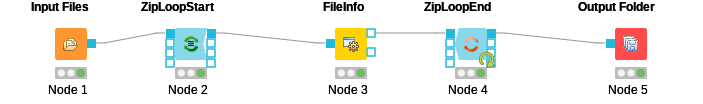
\includegraphics[width=\textwidth]{graphics/knime_setup/Minimal_FileInfoLoop}
\caption{A minimal workflow calling FileInfo on multiple files in a loop.}
\label{fig:knime_minimal_loop}
\end{figure}

\subsubsection{Advanced topic: Meta nodes}

Workflows can get rather complex and may contain dozens or even hundreds of nodes. KNIME provides a simple way to improve handling and clarity of large workflows:

\KNIMENODE{MetaNodes} allow to bundle several nodes into a single \KNIMENODE{Meta Node}.

\begin{task}
Select multiple nodes (e.g. all nodes of the ZipLoop including the start and end node). Open the context menu (right-click) and select \menu{Collapse into Meta Node}. Enter a caption for the \KNIMENODE{Meta Node}. The previously selected nodes are now contained in the \KNIMENODE{Meta Node}. Double clicking on the \KNIMENODE{Meta Node} will display the contained nodes in a new tab window. 
\end{task}

\begin{task}
Undo the packaging. First select the \KNIMENODE{Meta Node}, open the context menu (right-click) and select \menu{Expand Meta Node}.
\end{task}

\subsubsection{Advanced topic: R integration}

KNIME provides a large number of nodes for a wide range of statistical analysis, machine learning, data processing and visualization. Still, more recent statistical analysis methods, specialized visualizations or cutting edge algorithms may not be covered in KNIME. In order to expand its capabilities over the readily available nodes external scripting languages can be integrated. In this tutorial, we primarily use scripts of the powerful statistical computing language R. Note that this part is considered advanced and might be difficult to follow if you are not familiar with R. In this case you might skip this part.

\KNIMENODE{R View (Table)} allows to seamlessly include R scripts into KNIME. We will demonstrate on a minimal example how such a script is integrated.

\begin{task}
First we need some example data in KNIME, which we will generate using the \KNIMENODE{Data Generator} node. You can keep the default settings and execute the node. The table contains 4 columns, each containing random coordinates and one column containing a cluster number (Cluster\_0 to Cluster\_3). Now place a \KNIMENODE{R View (Table)} node into the workflow and connect the upper output port of the \KNIMENODE{Data Generator} node to the input of the \KNIMENODE{R View (Table)} node.
Right-click and configure the node.

If you get an error message like: Execute failed: R\_HOME does not contain a folder with name 'bin'. Please change the R settings in the preferences. To do so open \menu{File > Preferences > KNIME > R} and enter the path to your R installation (the folder that contains the bin directory).

If R is correctly recognized we can start writing an R script. Consider that we are interested in plotting the first and second coordinates and color them according to their cluster number. In R this can be done in a single line.

In the \KNIMENODE{R View (Table)} text editor, enter the following code:
\begin{lstlisting}
plot(x=knime.in$Universe_0_0, y=knime.in$Universe_0_1, main="Plotting column Universe_0_0 vs. Universe_0_1", col=knime.in$"Cluster Membership")
\end{lstlisting}
        
Explanation:
The table provided as input to the \KNIMENODE{R View (Table)} node is available as R \texttt{data.frame} with name \texttt{knime.in}. Columns (also listed on the left side of the R View window) can be accessed in the usual R way by first specifying the \texttt{data.frame} name and then the column name (e.g. \texttt{knime.in\$Universe\_0\_0)}.
\texttt{plot} is the plotting function we use to generate the image. We tell it to use the data in column \texttt{knime.in\$Universe\_0\_0} as x-coordinate and the column \texttt{knime.in\$Universe\_0\_1} as y coordinate in the plot. \texttt{main} is simply the plot name and col the column that is used to determine the color (in this case it is the \texttt{Cluster Membership} column).

Now press the \menu{Eval script} and \menu{Show plot} buttons.
\end{task}

\note{Note that we needed to put some extra quotes around \texttt{Cluster Membership}. If we omit those, R would interpret the column name only up to the first space (\texttt{knime.in\$Cluster}) which is not present in the table and leads to an error. Quotes are regularly needed if column names contain spaces or tabs.}


%!TEX root = handout.tex

\newpage
\section{Label-free quantification of metabolites}

\subsection{Introduction}
Quantitation and identification of chemical compounds are basic tasks in metabolomic studies. In this tutorial session we construct a UPLC-MS based, label-free quantitation and identification workflow. Following quantitation and identification we then perform statistical downstream analysis to detect quantitation values that differ significantly between two conditions. This approach can, for example, be used to detect biomarkers. Here, we use two spike-in conditions of a dilution series (0.5 mg/l and 10.0 mg/l, male blood background, measured in triplicates) comprising seven isotopically labeled compounds. The goal of this tutorial is to detect and quantify these differential spike-in compounds against the complex background.

%\begin{figure}[htbp]
%  \centering
%  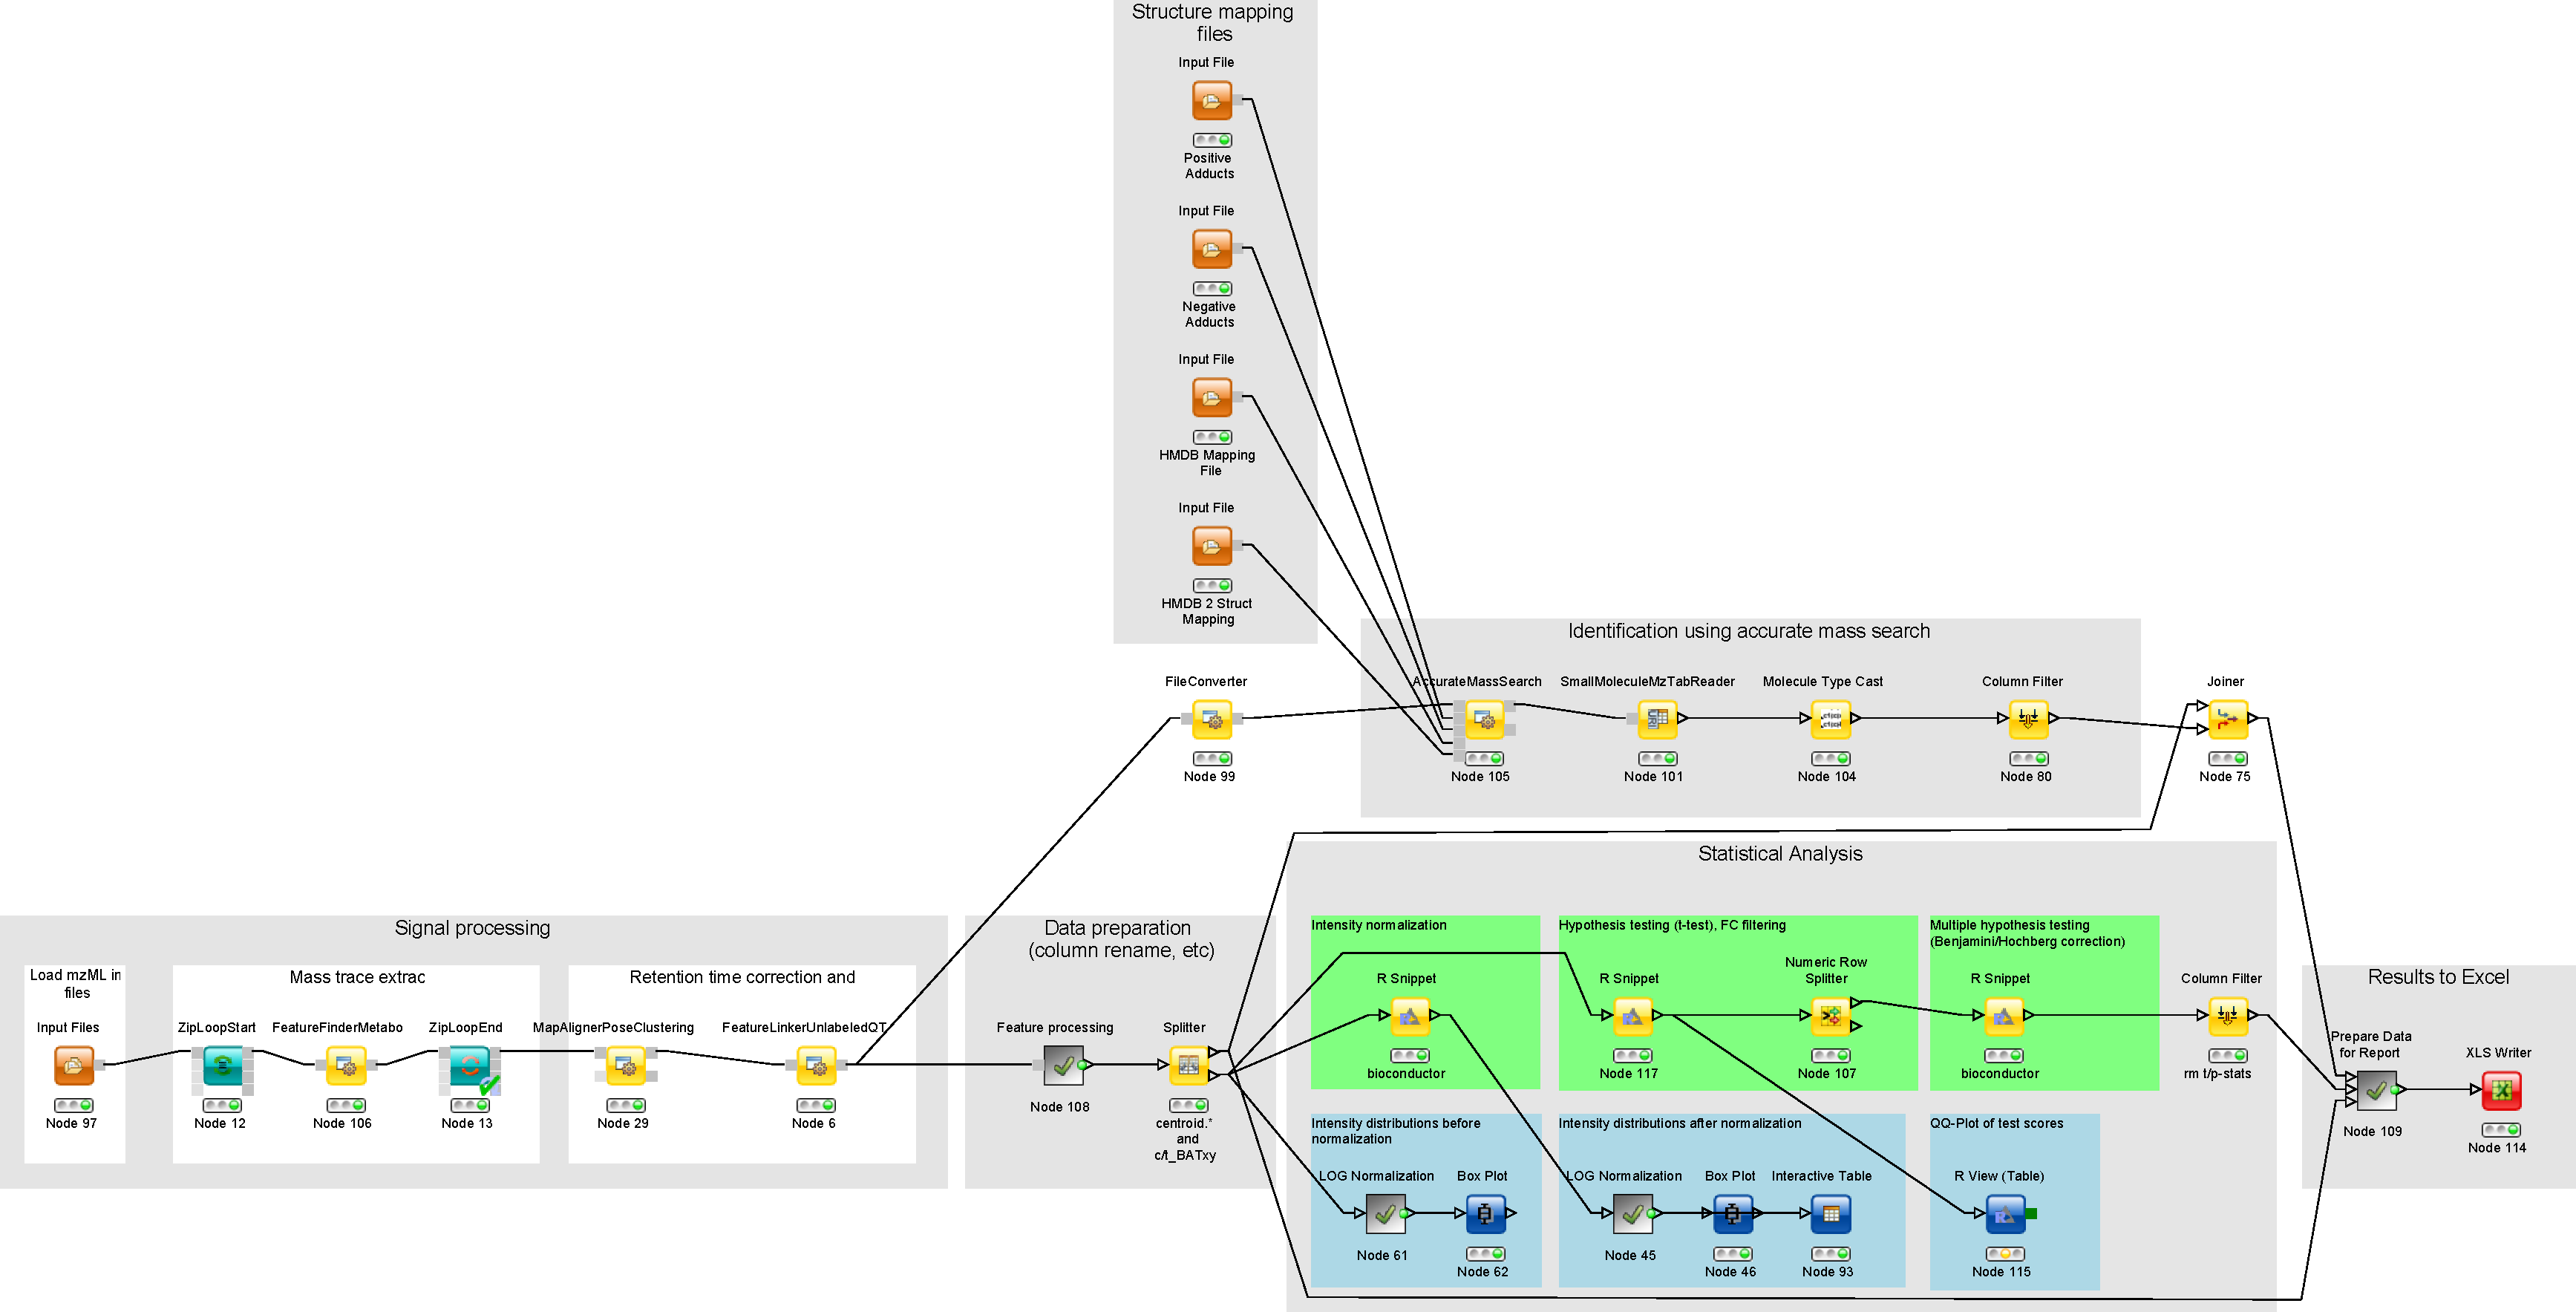
\includegraphics[width=0.85\textwidth]{graphics/metabo/metabo_workflow}
%  \caption{Complete label-free metabolomics quantification workflow}
%  \label{fig:consensusid}
%\end{figure}

\subsection{Basics of non-targeted metabolomics data analysis}

For the metabolite quantification we choose an approach similar to the one used for peptides, but this time based on the OpenMS \KNIMENODE{FeatureFinderMetabo} method. This feature finder again collects peak picked data into individual mass traces. The reason why we need a different feature finder for metabolites lies in the step after trace detection: the aggregation of isotopic traces belonging to the same compound ion into the same feature. Compared to peptides with their averagine model, small molecules have very different isotopic distributions. To group small molecule mass traces correctly, an aggregation model tailored to small molecules is thus needed. 

\begin{itemize}
\item
Create a new workflow called for instance "Metabolomics".
\item
Add an \KNIMENODE{Input File} node and configure it with one mzML file from the \directory{Example\_Data / Metabolomics / datasets}.
\item
Add a \KNIMENODE{FeatureFinderMetabo} node (from \menu{Community Nodes > OpenMS > Quantitation} and connect the first output port of the \KNIMENODE{Input File} to the \KNIMENODE{FeatureFinderMetabo}.
\item
For an optimal result adjust the following settings.
Please note that some of these are advanced parameters.
\item
Connect a \KNIMENODE{Output Folder} to the output of the \KNIMENODE{FeatureFinderMetabo} (see Fig.~\ref{fig:minimal_FFM_wf}).

\begin{figure}[!htbp]
  \centering
  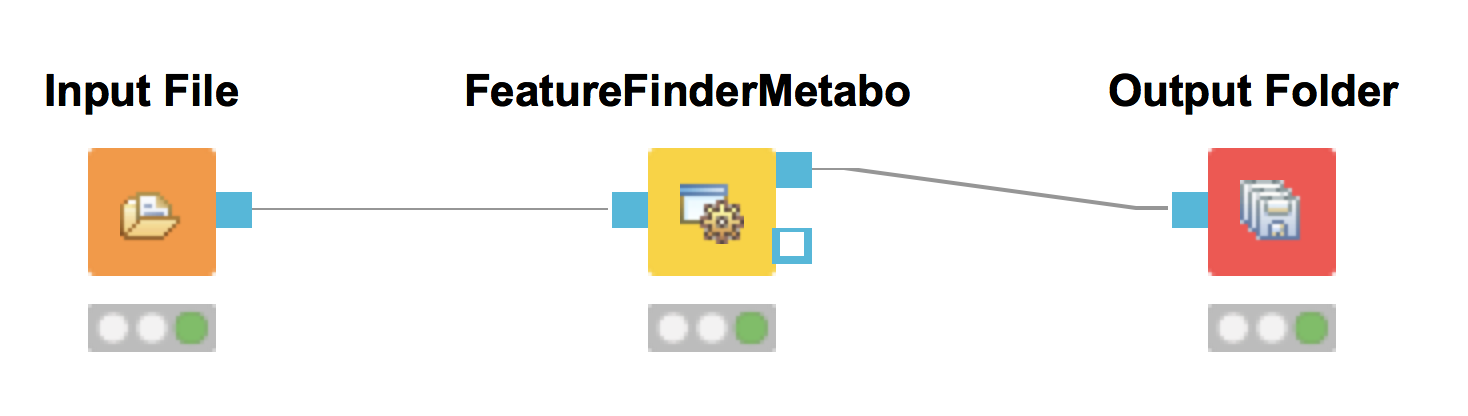
\includegraphics[width=0.5\textwidth]{graphics/metabo/minimal_FFM_wf.png}
  \caption{FeatureFinderMetabo workflow.}
  \label{fig:minimal_FFM_wf}
\end{figure}

In the following advanced parameters will be \hl{highlighted}. These parameter can be altered if the \menu{Show advanced parameter} field in the specific tool is activated (right bottom corner - see ~\ref{KNIME_concepts}). 

\begin{center}
\begin{tabular}{l|l}
\textbf{parameter} & \textbf{value} \\ \hline
\textit{algorithm $\rightarrow$ common $\rightarrow$ chrom\_fwhm} & $8.0$ \\
\textit{algorithm $\rightarrow$ mtd $\rightarrow$ trace\_termination\_criterion} & sample\_rate \\
\hl{\textit{algorithm $\rightarrow$ mtd $\rightarrow$ min\_trace\_length}} & $3.0$ \\
\hl{\textit{algorithm $\rightarrow$ mtd $\rightarrow$ max\_trace\_length}} & $600.0$\\
\textit{algorithm $\rightarrow$ epd $\rightarrow$ width\_filtering} & off \\
\textit{algorithm $\rightarrow$ ffm $\rightarrow$ report\_convex\_hulls} & true
\end{tabular}
\end{center}
\end{itemize}

The parameters change the behavior of \KNIMENODE{FeatureFinderMetabo} as follows:
\begin{itemize}
\item \textbf{chrom\_fwhm}: The expected chromatographic peak width in seconds.
\item \textbf{trace\_termination\_criterion}: In the first stage \KNIMENODE{FeatureFinderMetabo} assembles mass traces with a pre-defined mass accuracy. If this parameter is set to 'outlier', the extension of a mass trace is stopped after a predefined number of consecutive outliers is found. If this parameter is set to 'sample\_rate', the extension of a mass trace is stopped once the ratio of collected peaks versus visited spectra falls below the ratio given by min\_sample\_rate.
\item \textbf{min\_trace\_length}: Minimal length of a mass trace in seconds. Choose a small value, if you want to identify low-intensity compounds.
\item \textbf{max\_trace\_length}: Maximal length of a mass trace in seconds. Set this parameter to -1 to disable the filtering by maximal length.
\item \textbf{width\_filtering}: \KNIMENODE{FeatureFinderMetabo} can remove features with unlikely peak widths from the results. If activated it will use the interval provided by the paramters min\_fwhm and max\_fwhm.
\item \textbf{report\_convex\_hulls}: If set to true, convex hulls including mass traces will be reported for all identified features. This increases the output size considerably.
\end{itemize}

\noindent The output file .featureXML can be visualized with TOPPView on top of the used .mzML file - in a so called 	\textit{layer} - to look at the identified features.
\newline
 
\noindent First start TOPPView and open the example .mzML file (see Fig.~\ref{fig:ToppView_1}). Afterwards open the .featureXML output as new layer (see Fig.~\ref{fig:ToppView_2}). The overlay is depcied in Figure~\ref{fig:ToppView_3}. The zoom of the .mzML - .featureXML overlay shows the individual mass traces and the assembly of those in a feature (see Fig.~\ref{fig:ToppView_4}).

\begin{figure}[htbp]
  \centering
  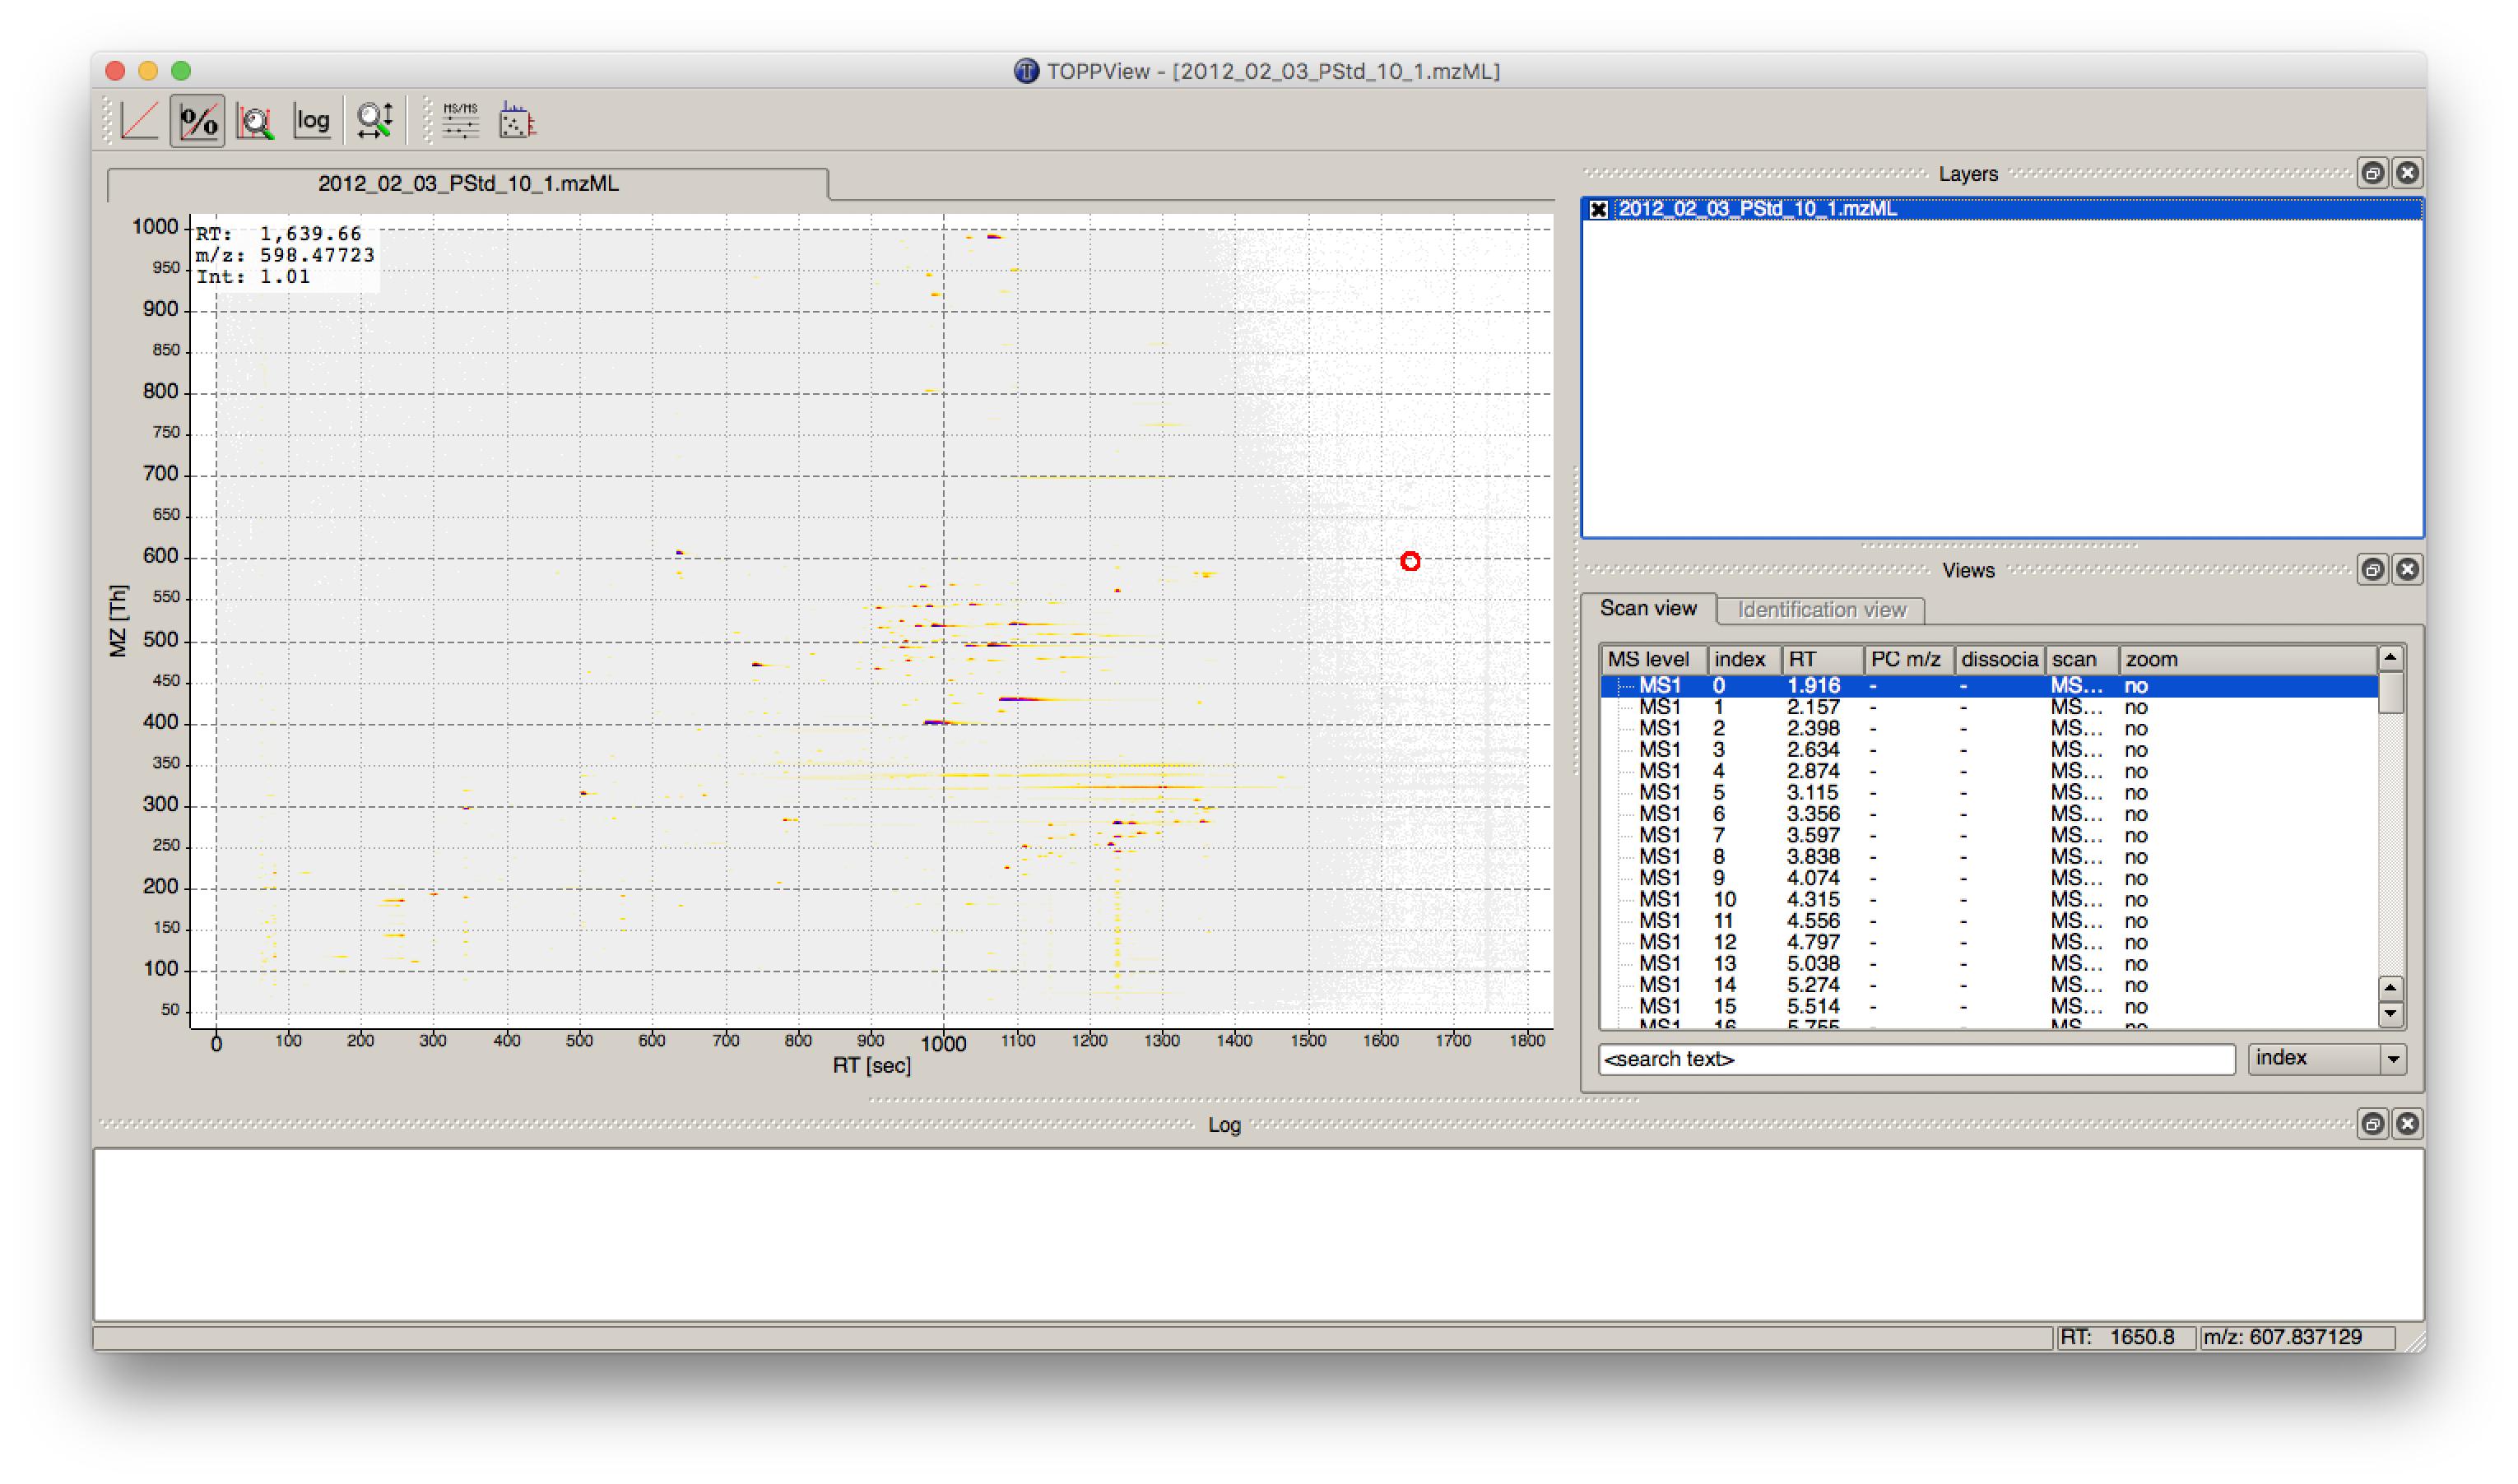
\includegraphics[width=\textwidth]{graphics/metabo/ToppView_1.png}
  \caption{Openend .mzML in TOPPView.}
  \label{fig:ToppView_1}
\end{figure}

\begin{figure}[htbp]
  \centering
  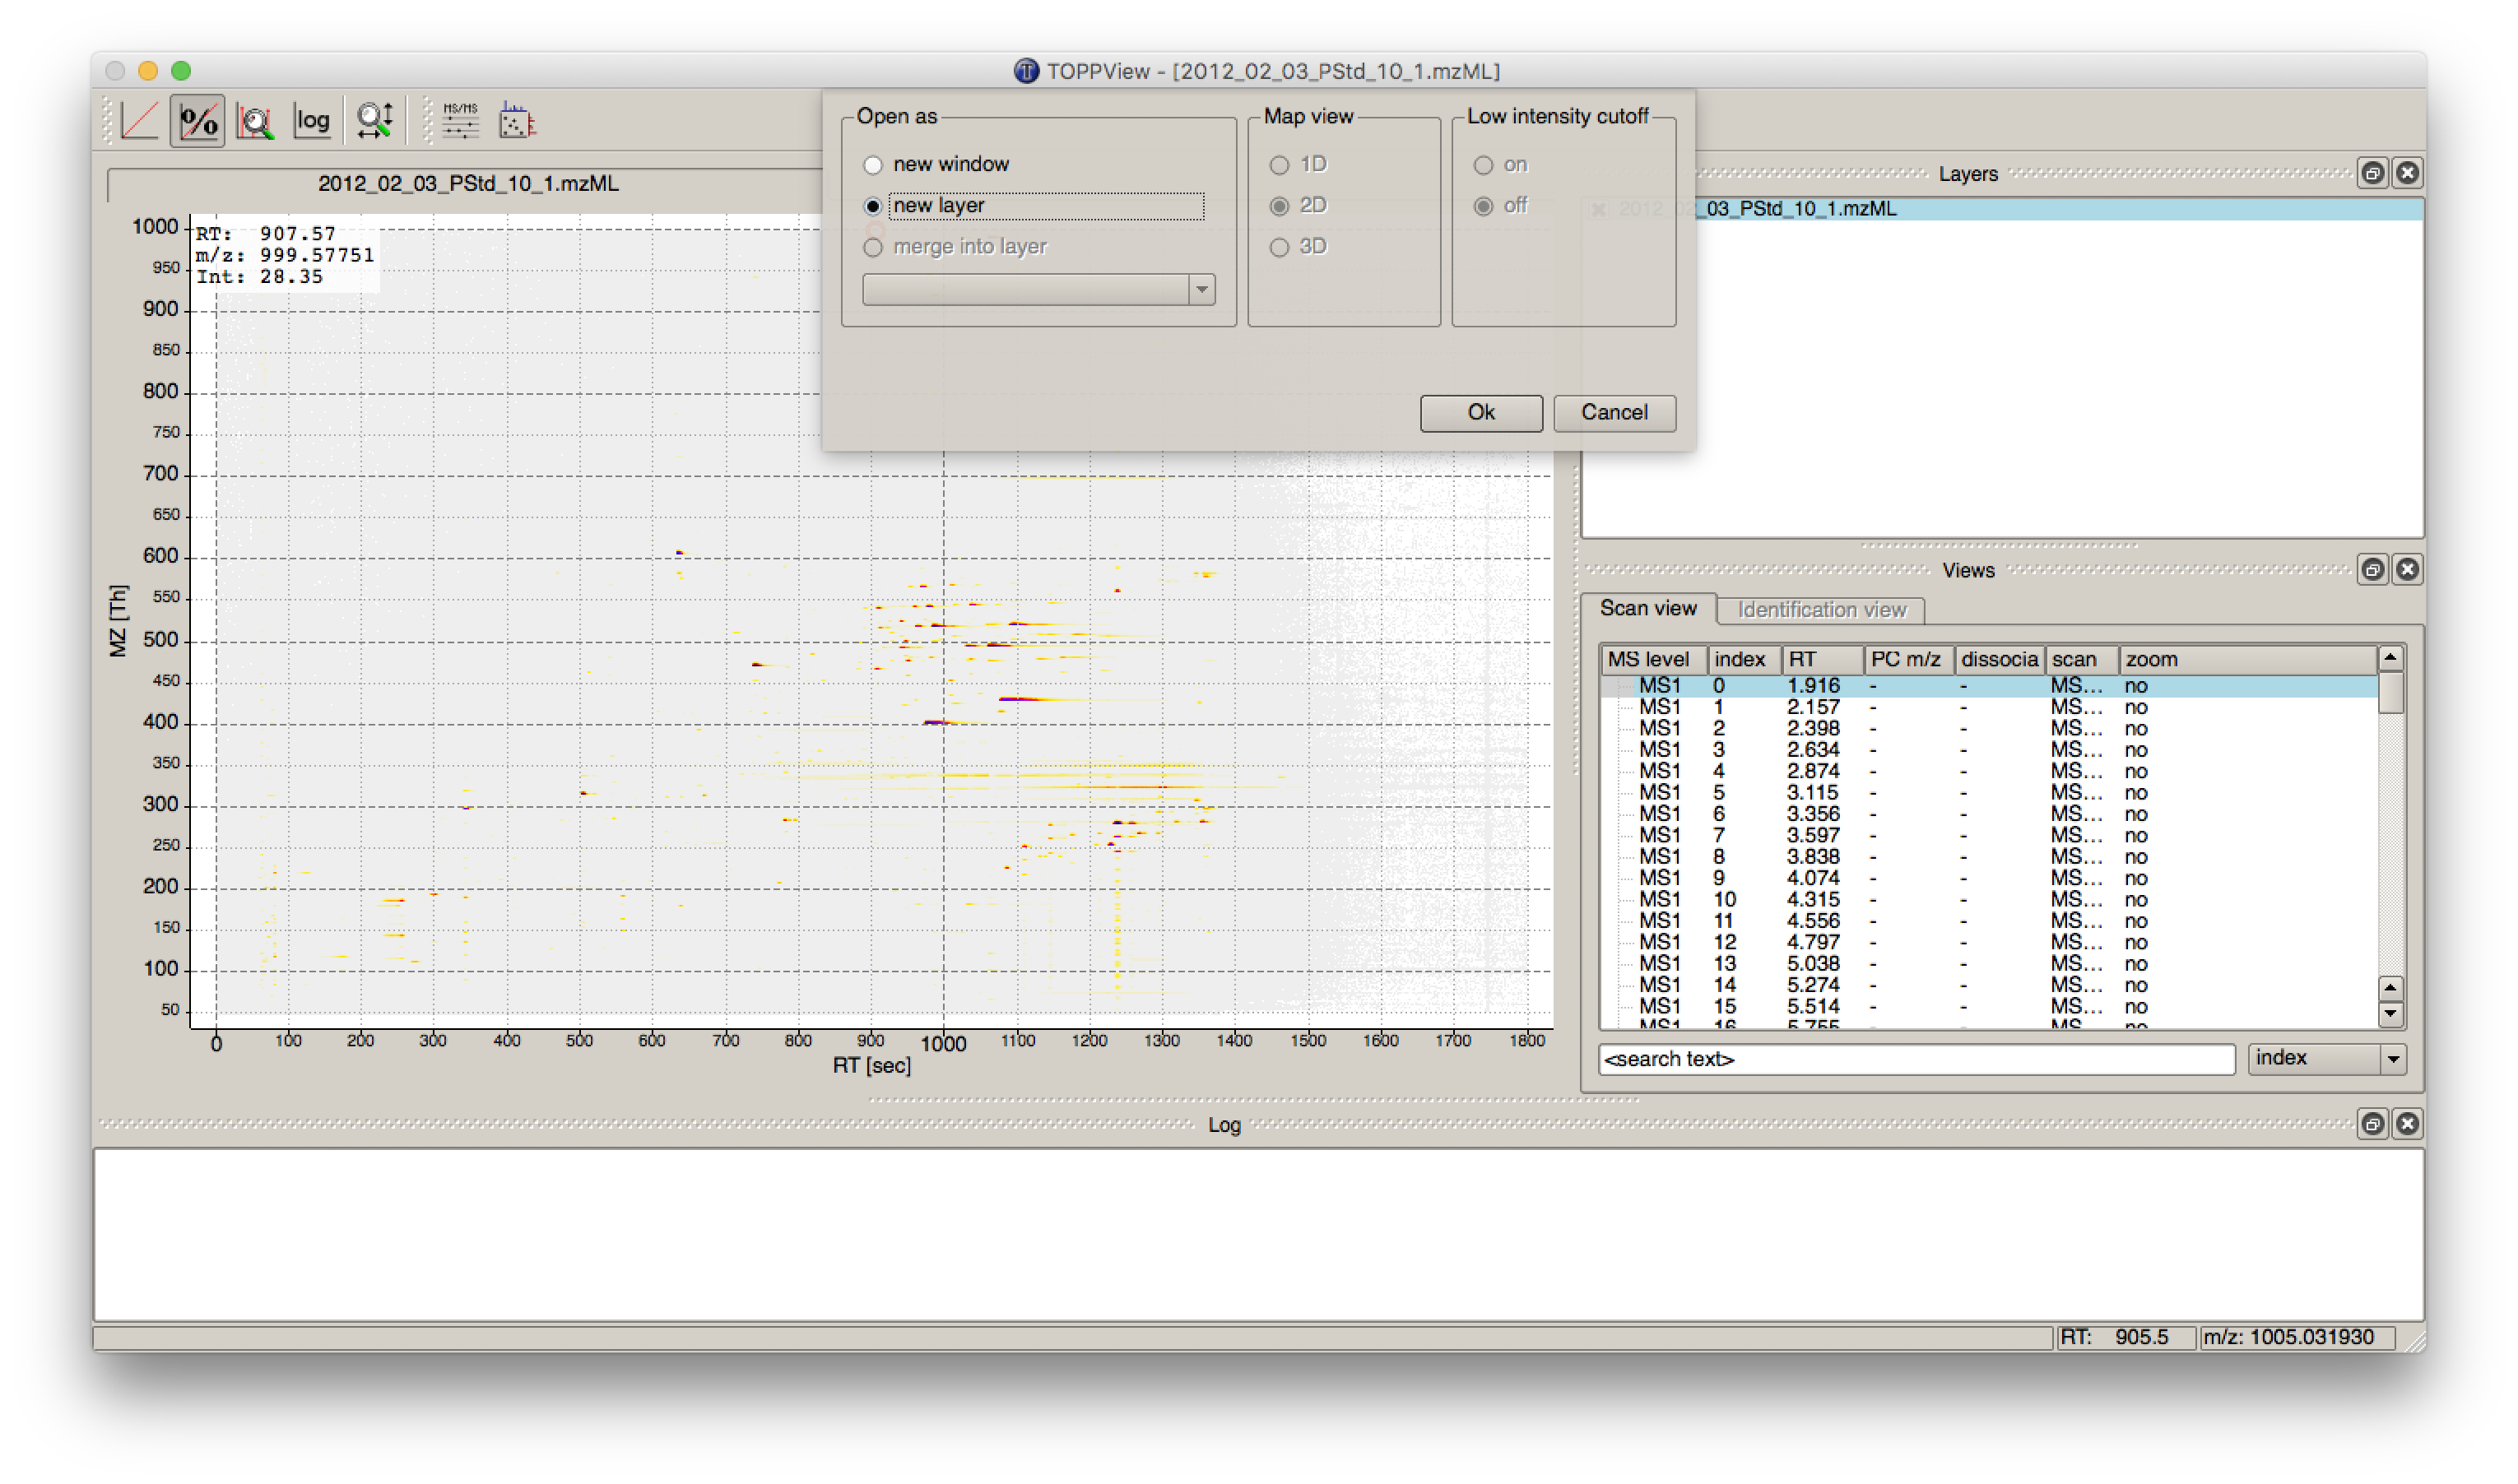
\includegraphics[width=\textwidth]{graphics/metabo/ToppView_2.png}
  \caption{Add new layer in TOPPView.}
  \label{fig:ToppView_2}
\end{figure}

\begin{figure}[htbp]
  \centering
  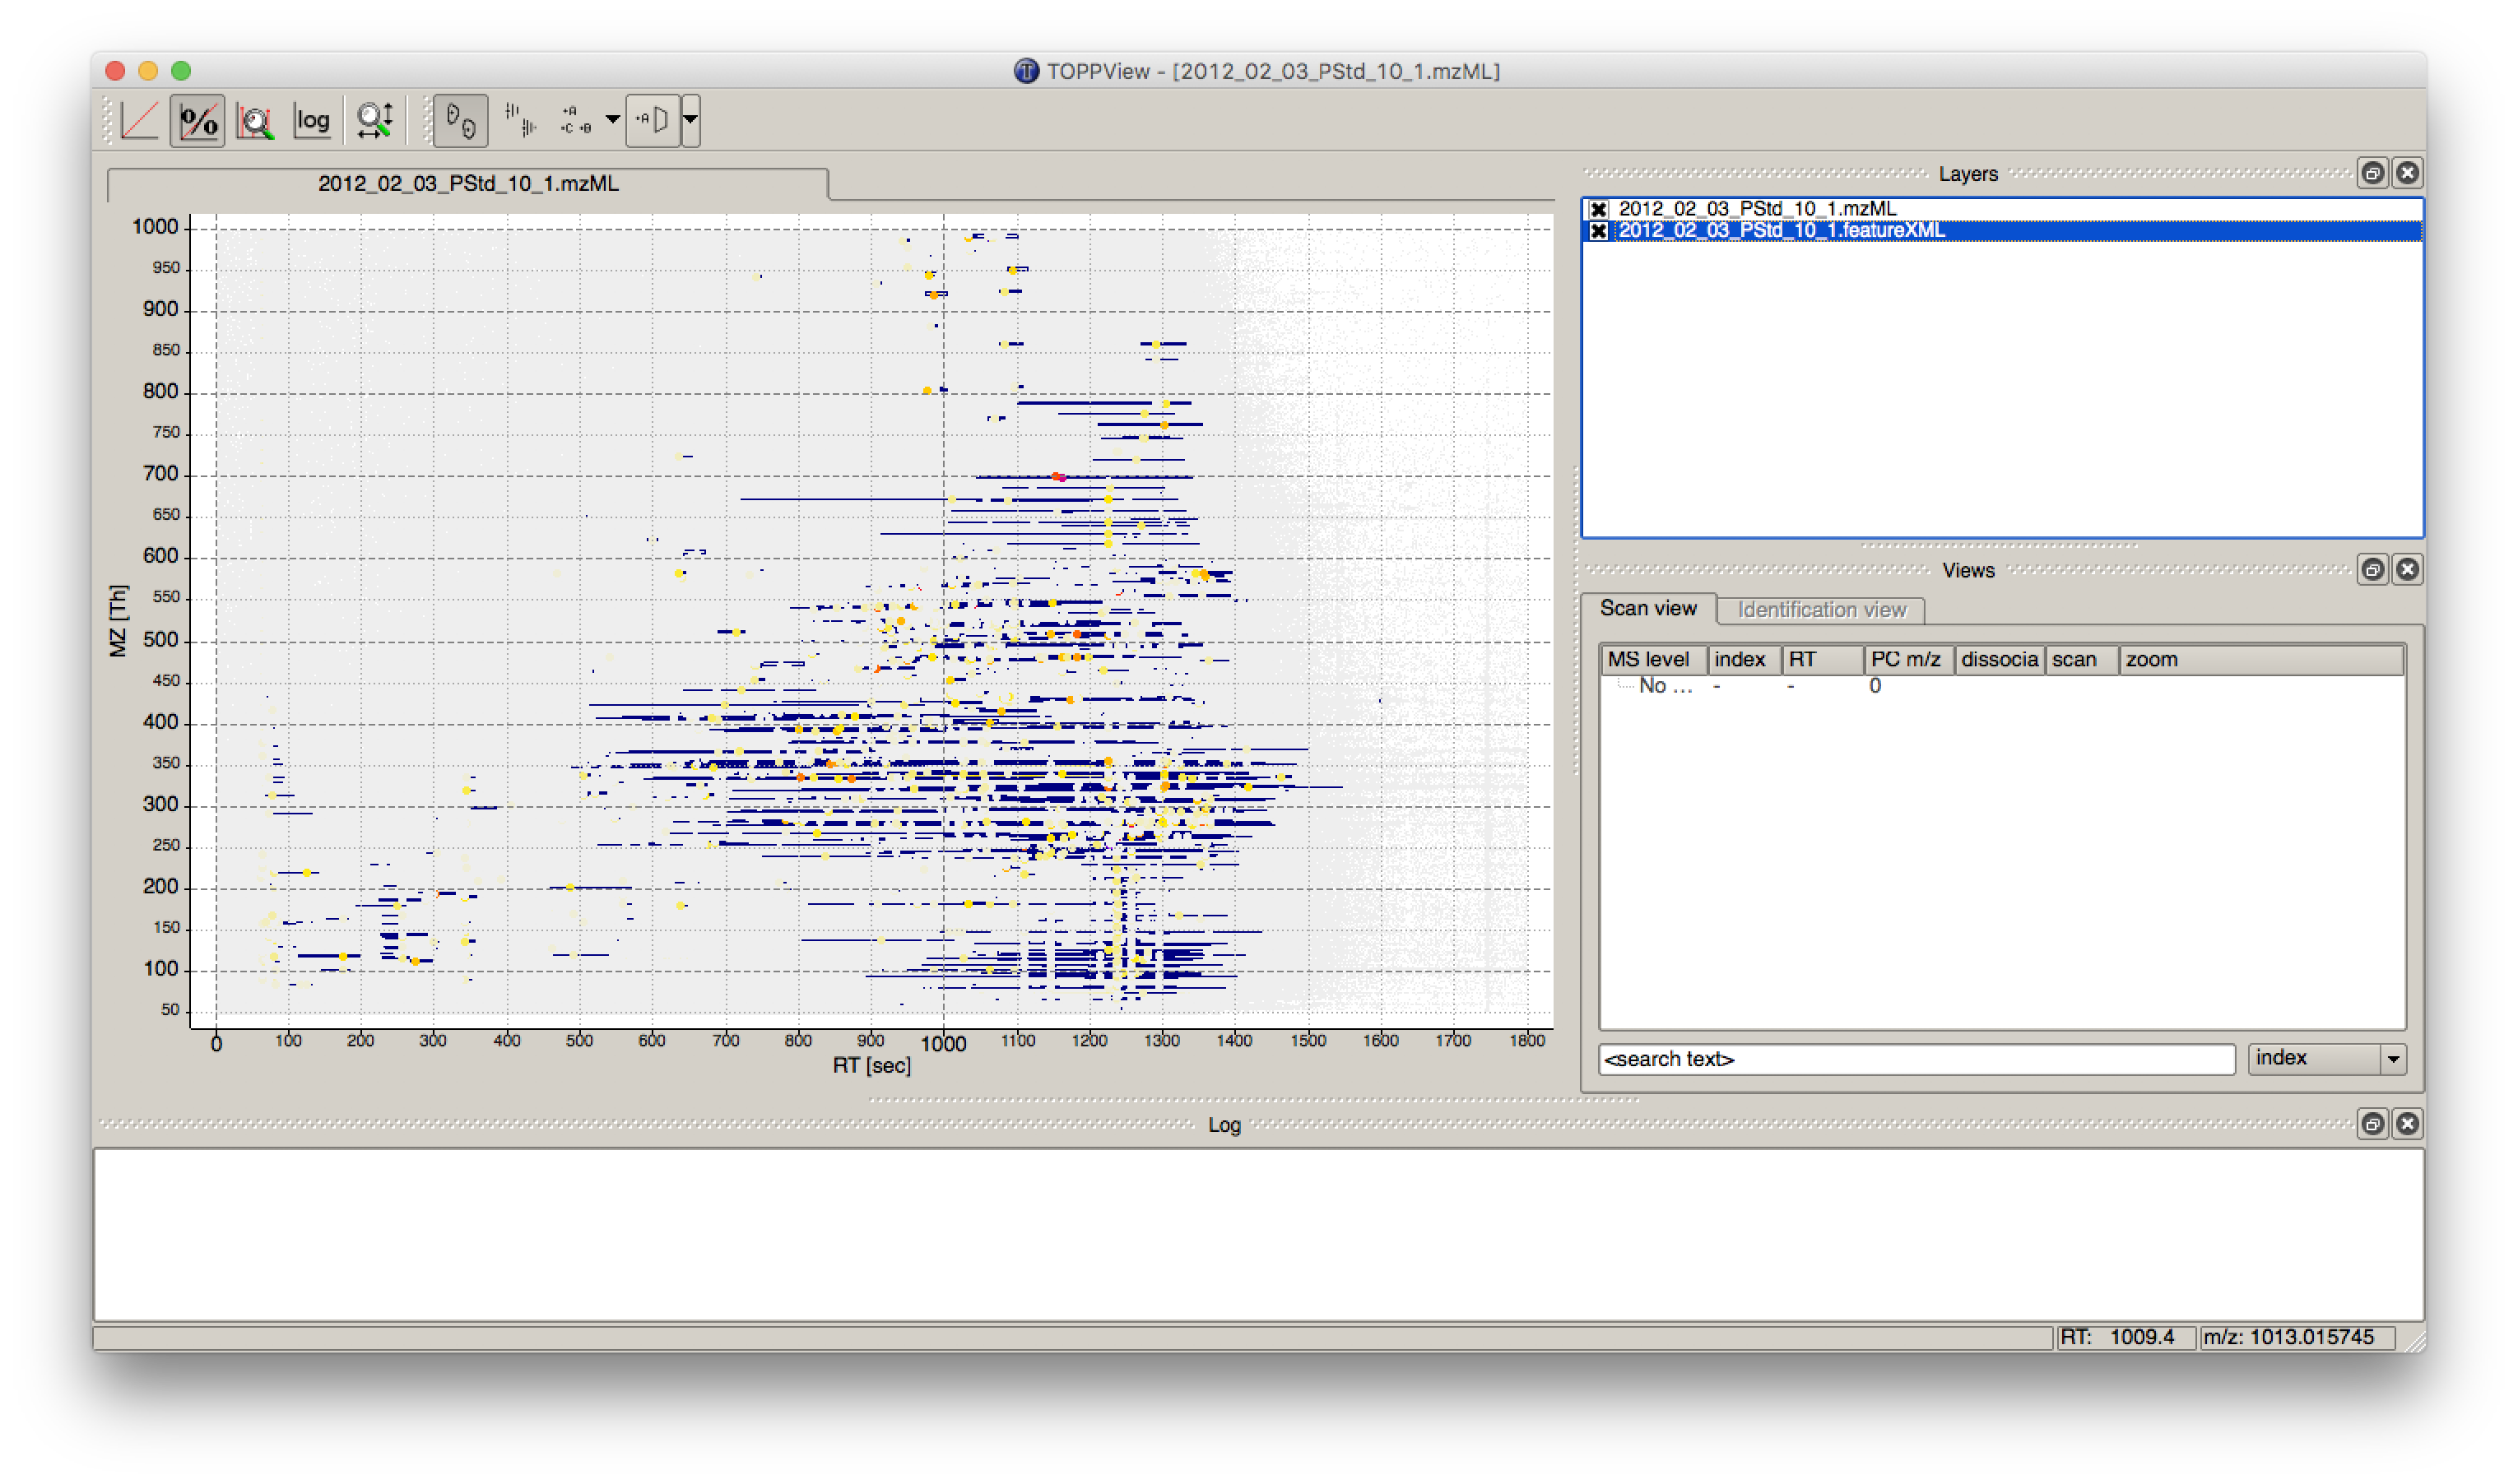
\includegraphics[width=\textwidth]{graphics/metabo/ToppView_3.png}
  \caption{Overlay of the .mzML layer with the .featureXML layer. }
  \label{fig:ToppView_3}
\end{figure}

\begin{figure}[htbp]
  \centering
  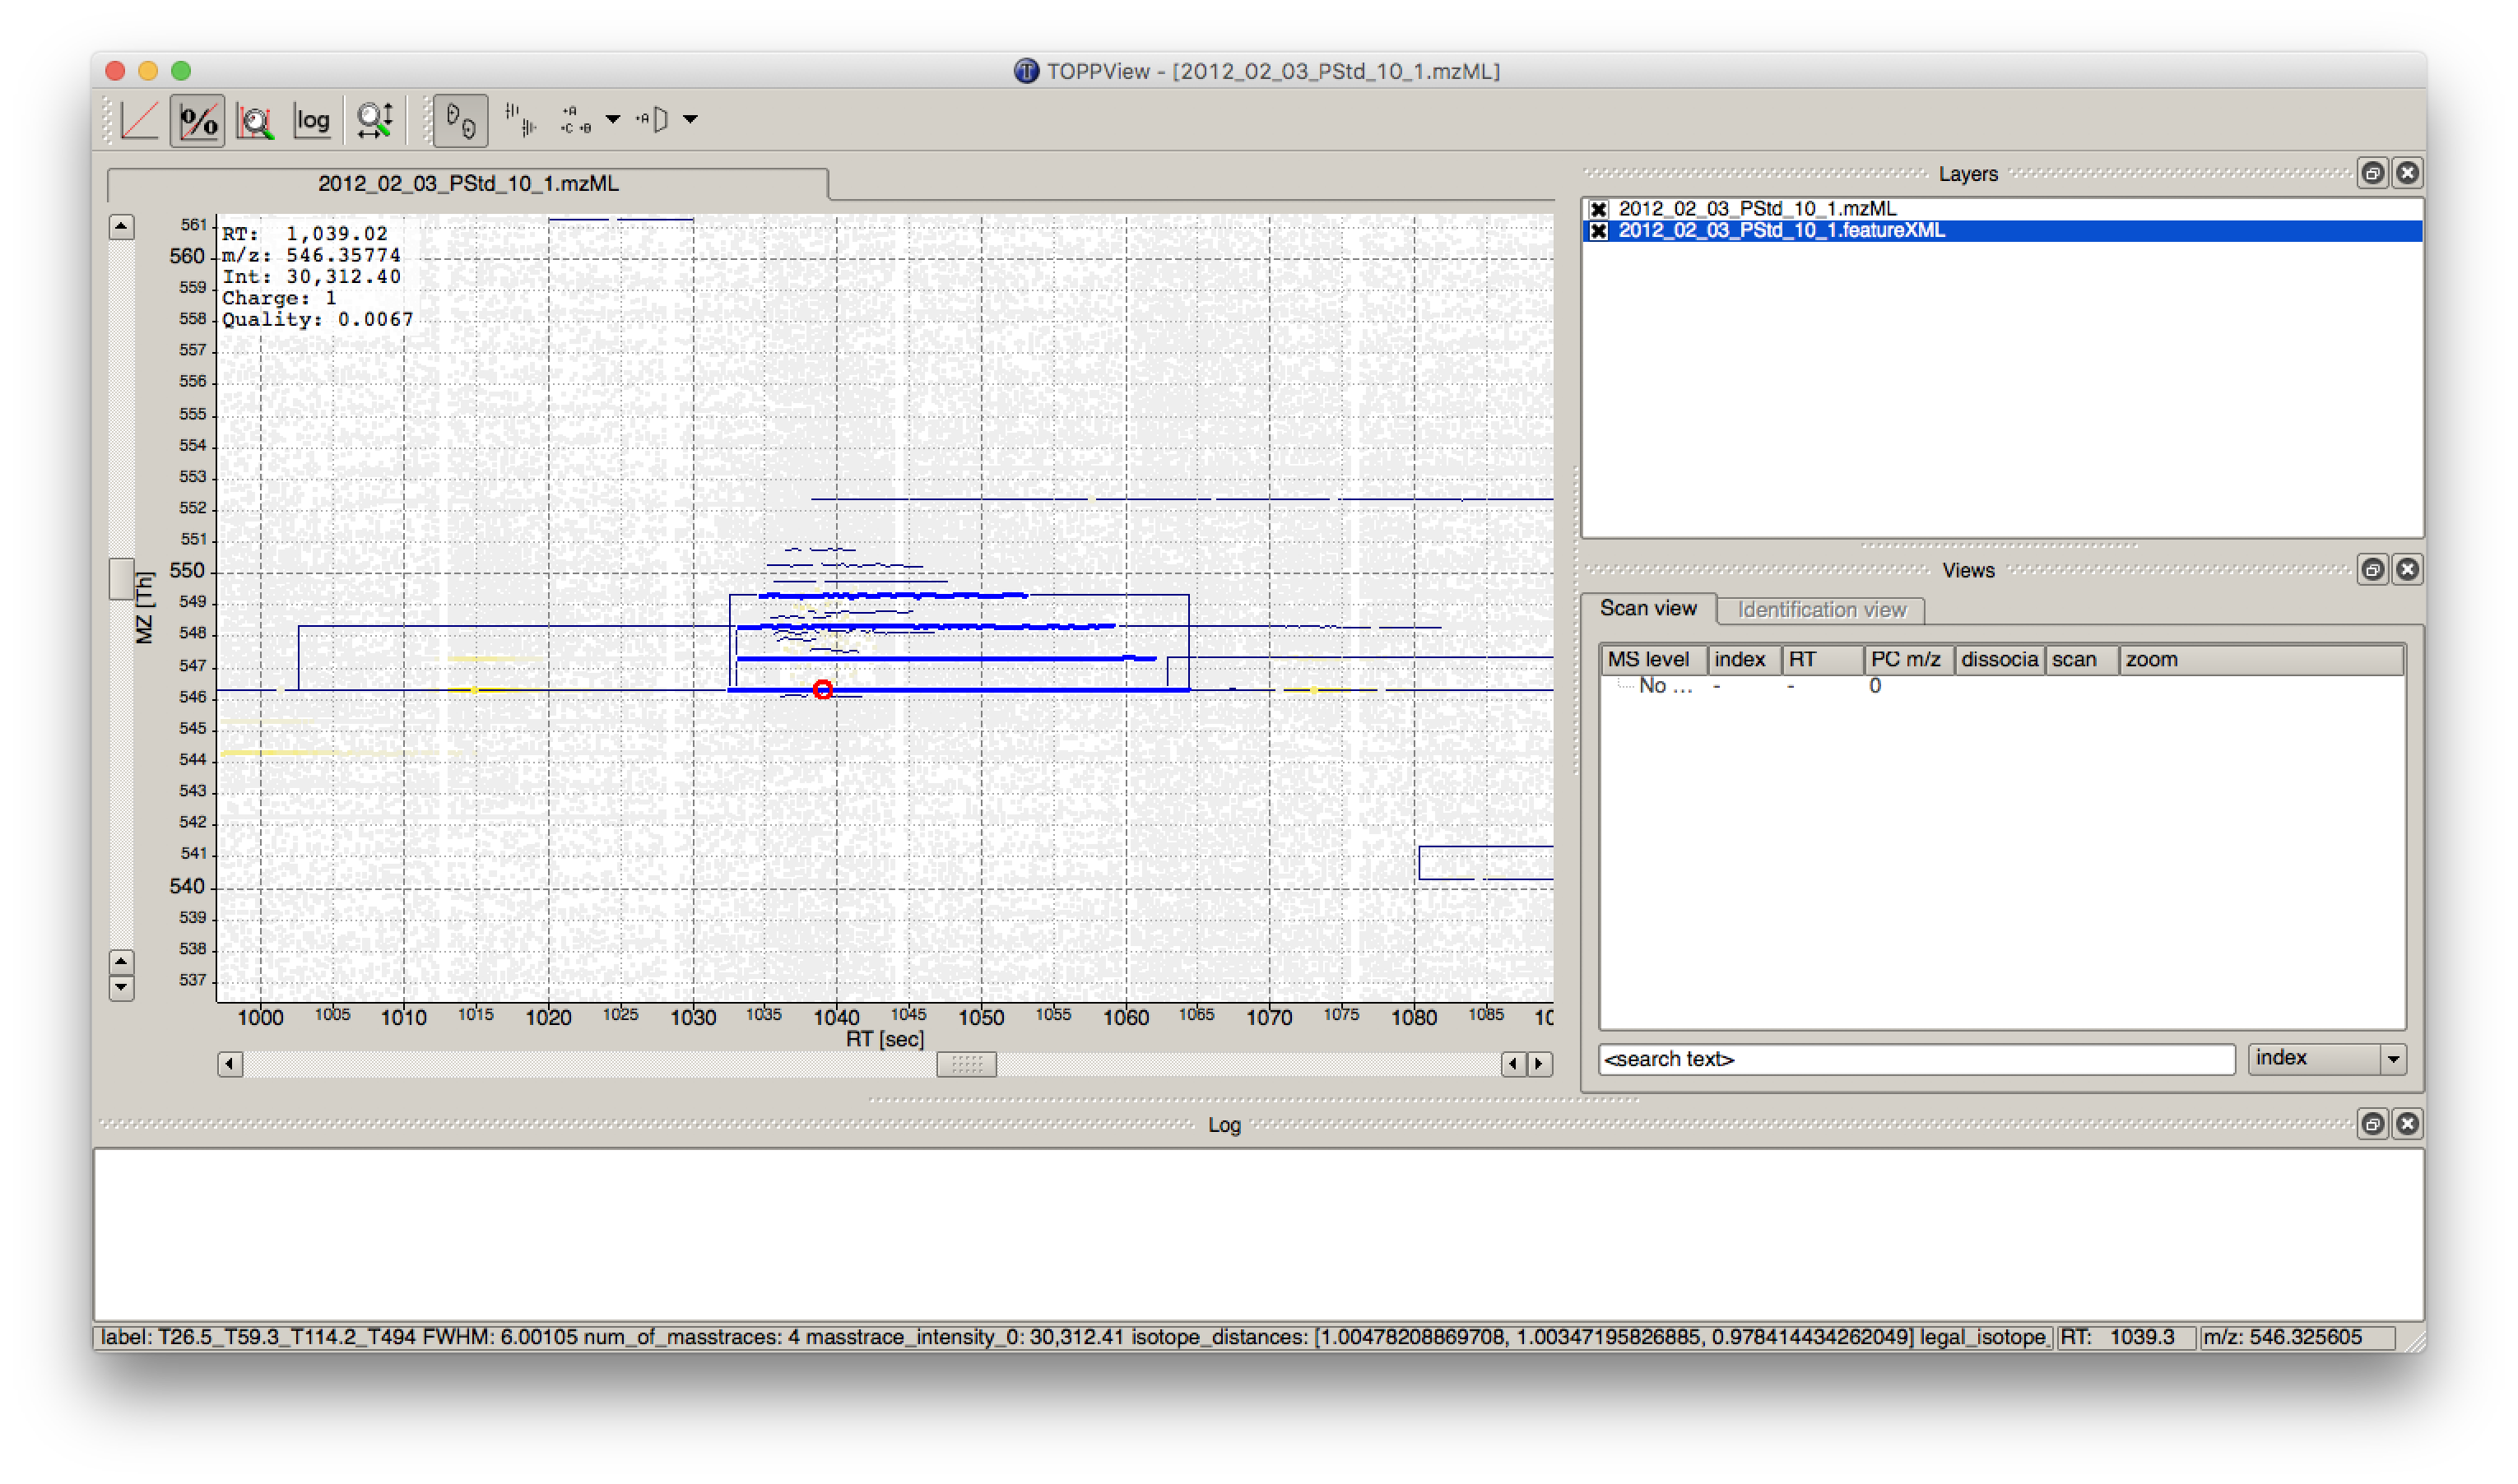
\includegraphics[width=\textwidth]{graphics/metabo/ToppView_4.png}
  \caption{Zoom of the overlay of the .mzML with the .featureXML layer. Here the individual isotope traces (blue lines) are assembled into a feature here shown as convex hull (rectangular box).}
  \label{fig:ToppView_4}
\end{figure}

The workflow can be extended for multi-file analysis, here an \KNIMENODE{Input Files} is to be used instead of the \KNIMENODE{Input File}.  In front of the \KNIMENODE{FeatureFinderMetabo} a \KNIMENODE{Ziploop Start} and behind \KNIMENODE{Ziploop End} has to be used, since FeatureFinderMetabo will analyis on file to file bases. 
\newline
To facilitate the collection of features corresponding to the same compound ion across different samples, an alignment of the samples' feature maps along retention time is often helpful. In addition to local, small-scale elution differences, one can often see constant retention time shifts across large sections between samples. We can use linear transformations to correct for these large scale retention differences. This  brings the majority of corresponding compound ions close to each other. Finding the correct corresponding ions is then faster and easier, as we don't have to search as far around individual features.

\begin{figure}[!htbp]
	\centering
	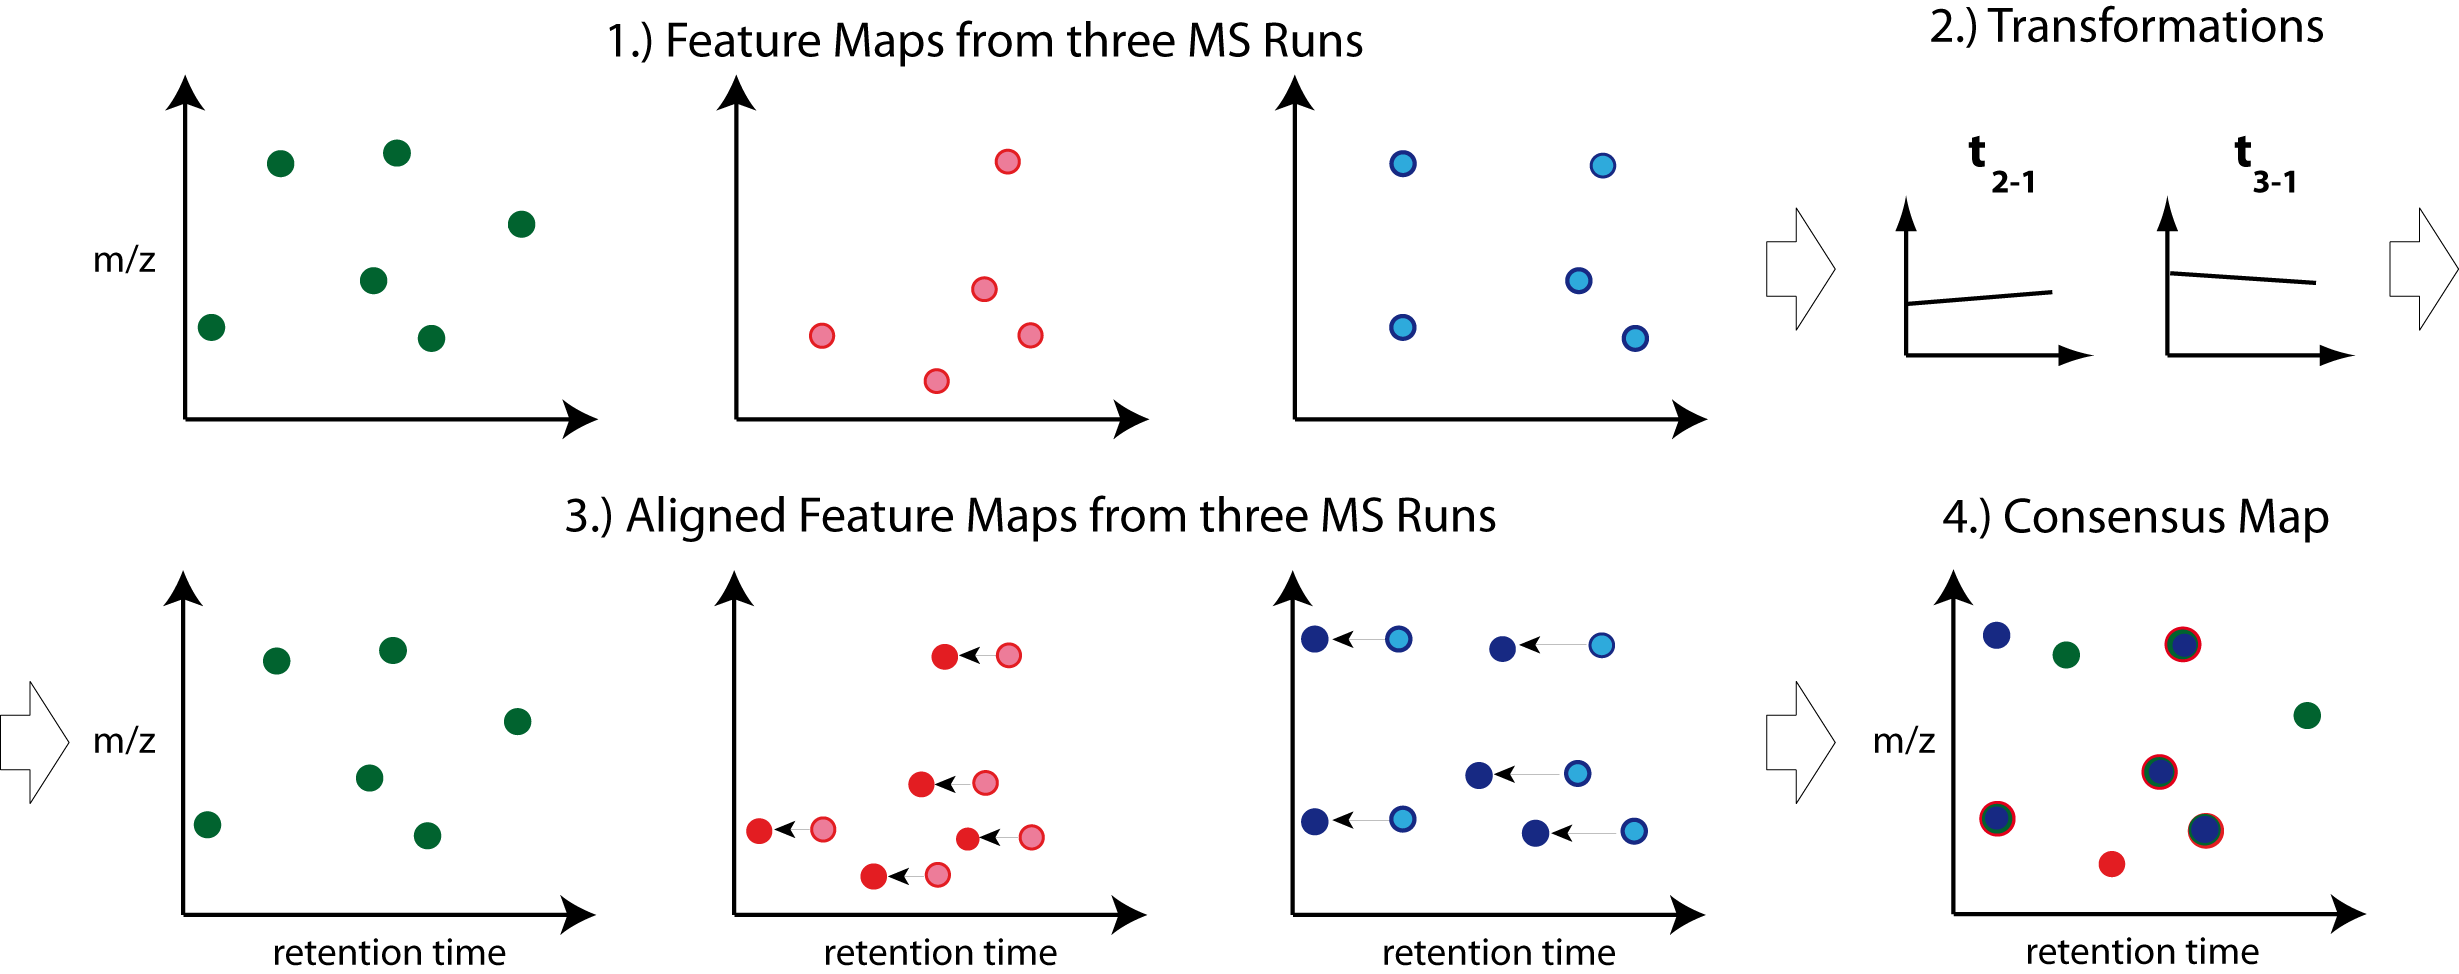
\includegraphics[width=\textwidth]{graphics/metabo/align.png}
	\caption[Map alignment]
	{
	\textbf{Map alignment.} The first feature map is used as a reference to which other maps are aligned. The calculated transformation brings corresponding features into close retention time proximity. Linking of these features form a so-called consensus features of a \textit{consensus map}.
	}
	\label{bg_alignment}
\end{figure}

\begin{itemize}
\item
After the \KNIMENODE{ZipLoopEnd} node add a \KNIMENODE{MapAlignerPoseClustering} node (\menu{Community Nodes > OpenMS > Map Alignment}), set its Output Type to featureXML, and adjust the following settings

\begin{center}
\begin{tabular}{l|l}
\textbf{parameter} & \textbf{value} \\ \hline
\textit{algorithm $\rightarrow$ max\_num\_peaks\_considered} & $-1$ \\
\textit{algorithm $\rightarrow$ superimposer $\rightarrow$ mz\_pair\_max\_distance} & $0.005$ \\
\textit{algorithm $\rightarrow$ superimposer $\rightarrow$ num\_used\_points} & $10000$ \\
\textit{algorithm $\rightarrow$ pairfinder $\rightarrow$ distance\_RT $\rightarrow$ max\_difference} & $20.0$ \\
\textit{algorithm $\rightarrow$ pairfinder $\rightarrow$ distance\_MZ $\rightarrow$ max\_difference} & $20.0$ \\
\textit{algorithm $\rightarrow$ pairfinder $\rightarrow$ distance\_MZ $\rightarrow$ unit} & ppm
\end{tabular}
\end{center}

\end{itemize}

\noindent \KNIMENODE{MapAlignerPoseClustering} provides an algorithm to align the retention time scales of multiple input files, correcting shifts and distortions between them. Retention time adjustment may be necessary to correct for chromatography differences e.g. before data from multiple LC-MS runs can be combined (feature linking). The alignment algorithm implemented here is the pose clustering algorithm. \\

\noindent The parameters change the behavior of \KNIMENODE{MapAlignerPoseClustering} as follows:
\begin{itemize}
\item \textbf{max\_num\_peaks\_considered}: The maximal number of peaks/features to be considered per map. To use all, set this parameter to -1.
\item \textbf{mz\_pair\_max\_distance}: Maximum of m/z deviation of corresponding elements in different maps.  This condition applies to the pairs considered in hashing.
\item \textbf{num\_used\_points}: Maximum number of elements considered in each map (selected by intensity). Use a smaller number to reduce the running time and to disregard weak signals during alignment.
\item \textbf{distance\_RT $\rightarrow$ max\_difference}: Features that have a larger RT difference will never be paired.
\item \textbf{distance\_MZ $\rightarrow$ max\_difference}: Features that have a larger m/z difference will never be paired.
\item \textbf{distance\_MZ $\rightarrow$ unit}: Unit used for the parameter distance\_MZ max\_difference, either Da or ppm.
\end{itemize}

The next step after retention time correction is the grouping of corresponding features in multiple samples. In contrast to the previous alignment, we assume no linear relations of features across samples. The used method is tolerant against local swaps in elution order.

\begin{figure}[htb]
	\centering
	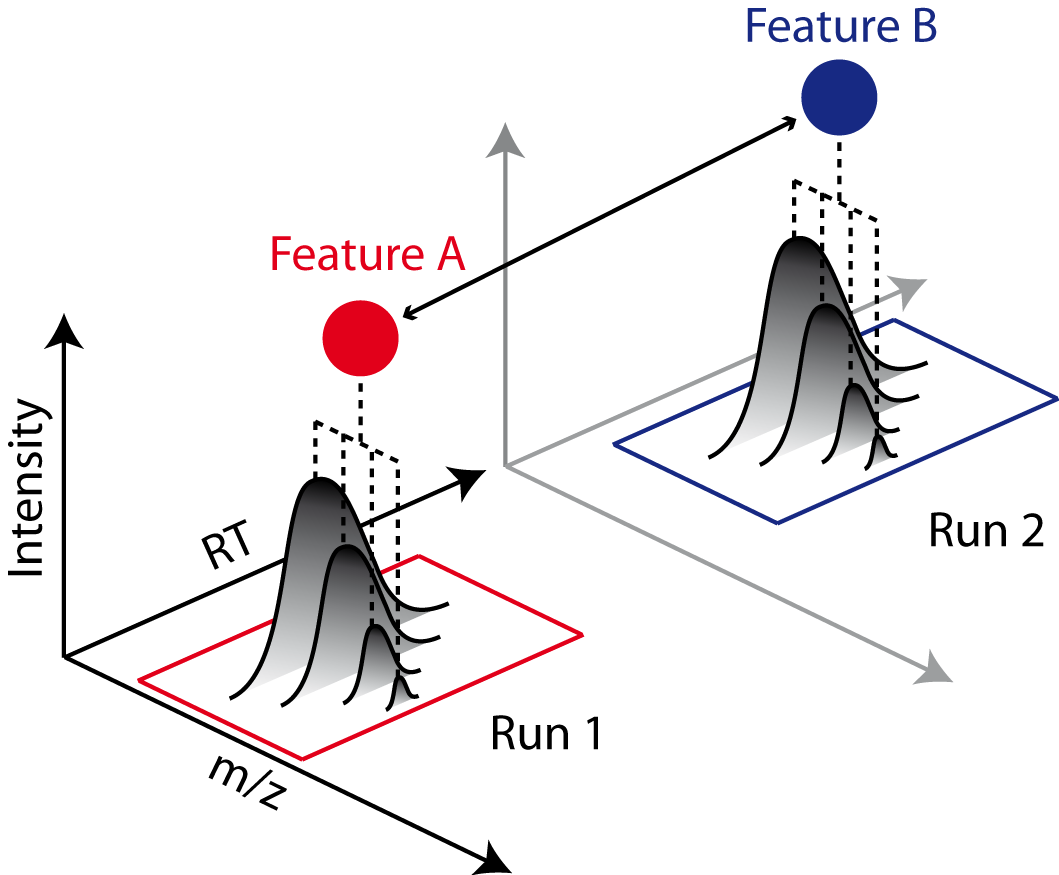
\includegraphics[width=0.7\textwidth]{graphics/metabo/link.png}
	\caption[Label-free quantification]
	{
	\textbf{Feature linking}. Features A and B correspond to the same analyte. The linking of features between runs (indicated by an arrow) allows comparing feature intensities.
	}
	\label{fig_bg_link}
\end{figure}

\begin{itemize}
\item
After the \KNIMENODE{MapAlignerPoseClustering} add a \KNIMENODE{FeatureLinkerUnlabeledQT} \\
 (\menu{Community Nodes > OpenMS > Map Alignment}) and adjust the following settings

\begin{center}
\begin{tabular}{l|l}
\textbf{parameter} & \textbf{value} \\ \hline
\textit{algorithm $\rightarrow$ distance\_RT $\rightarrow$ max\_difference} & $40.0$ \\
\textit{algorithm $\rightarrow$ distance\_MZ $\rightarrow$ max\_difference} & $20.0$ \\
\textit{algorithm $\rightarrow$ distance\_MZ $\rightarrow$ unit} & ppm
\end{tabular}
\end{center}

\noindent The parameters change the behavior of \KNIMENODE{FeatureLinkerUnlabeledQT} as follows (similar to the parameters we adjusted for \KNIMENODE{MapAlignerPoseClustering}):
\begin{itemize}
\item \textbf{distance\_RT $\rightarrow$ max\_difference}: Features that have a larger RT difference will never be paired.
\item \textbf{distance\_MZ $\rightarrow$ max\_difference}: Features that have a larger m/z difference will never be paired.
\item \textbf{distance\_MZ $\rightarrow$ unit}: Unit used for the parameter distance\_MZ max\_difference, either Da or ppm.
\end{itemize}

\item
After the \KNIMENODE{FeatureLinkerUnlabeledQT} add a \KNIMENODE{TextExporter} node (\menu{Community Nodes > OpenMS > File Handling}).
\item
Add an \KNIMENODE{Output Folder} node and configure it with an output directory where you want to store the resulting files.
\item
Run the pipeline and inspect the output.
\end{itemize}

\begin{figure}[htbp]
  \centering
  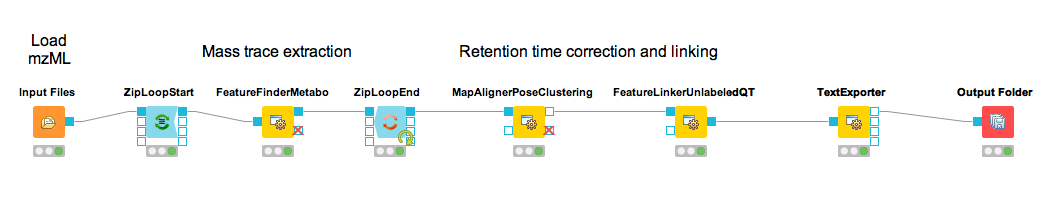
\includegraphics[width=0.85\textwidth]{graphics/metabo/metabo_part1_with_labels.png}
  \caption{Label-free quantification workflow for metabolites}
  \label{fig:metabo_part1}
\end{figure}

You should find a single, tab-separated file containing the information on where metabolites were found and with which intensities.
You can also add \KNIMENODE{Output Folder} nodes at different stages of the workflow and inspect the intermediate results (e.g., identified metabolite features for each input map).
The complete workflow can be seen in \cref{fig:metabo_part1}.
In the following section we will try to identify those metabolites.

\noindent The \KNIMENODE{FeatureLinkerUnlabeledQT} output can be visualized in ToppView on top of the input and output of the \KNIMENODE{FeatureFinderMetabo} (see Fig~\ref{fig:ToppView_5}). 

\begin{figure}[htbp]
  \centering
  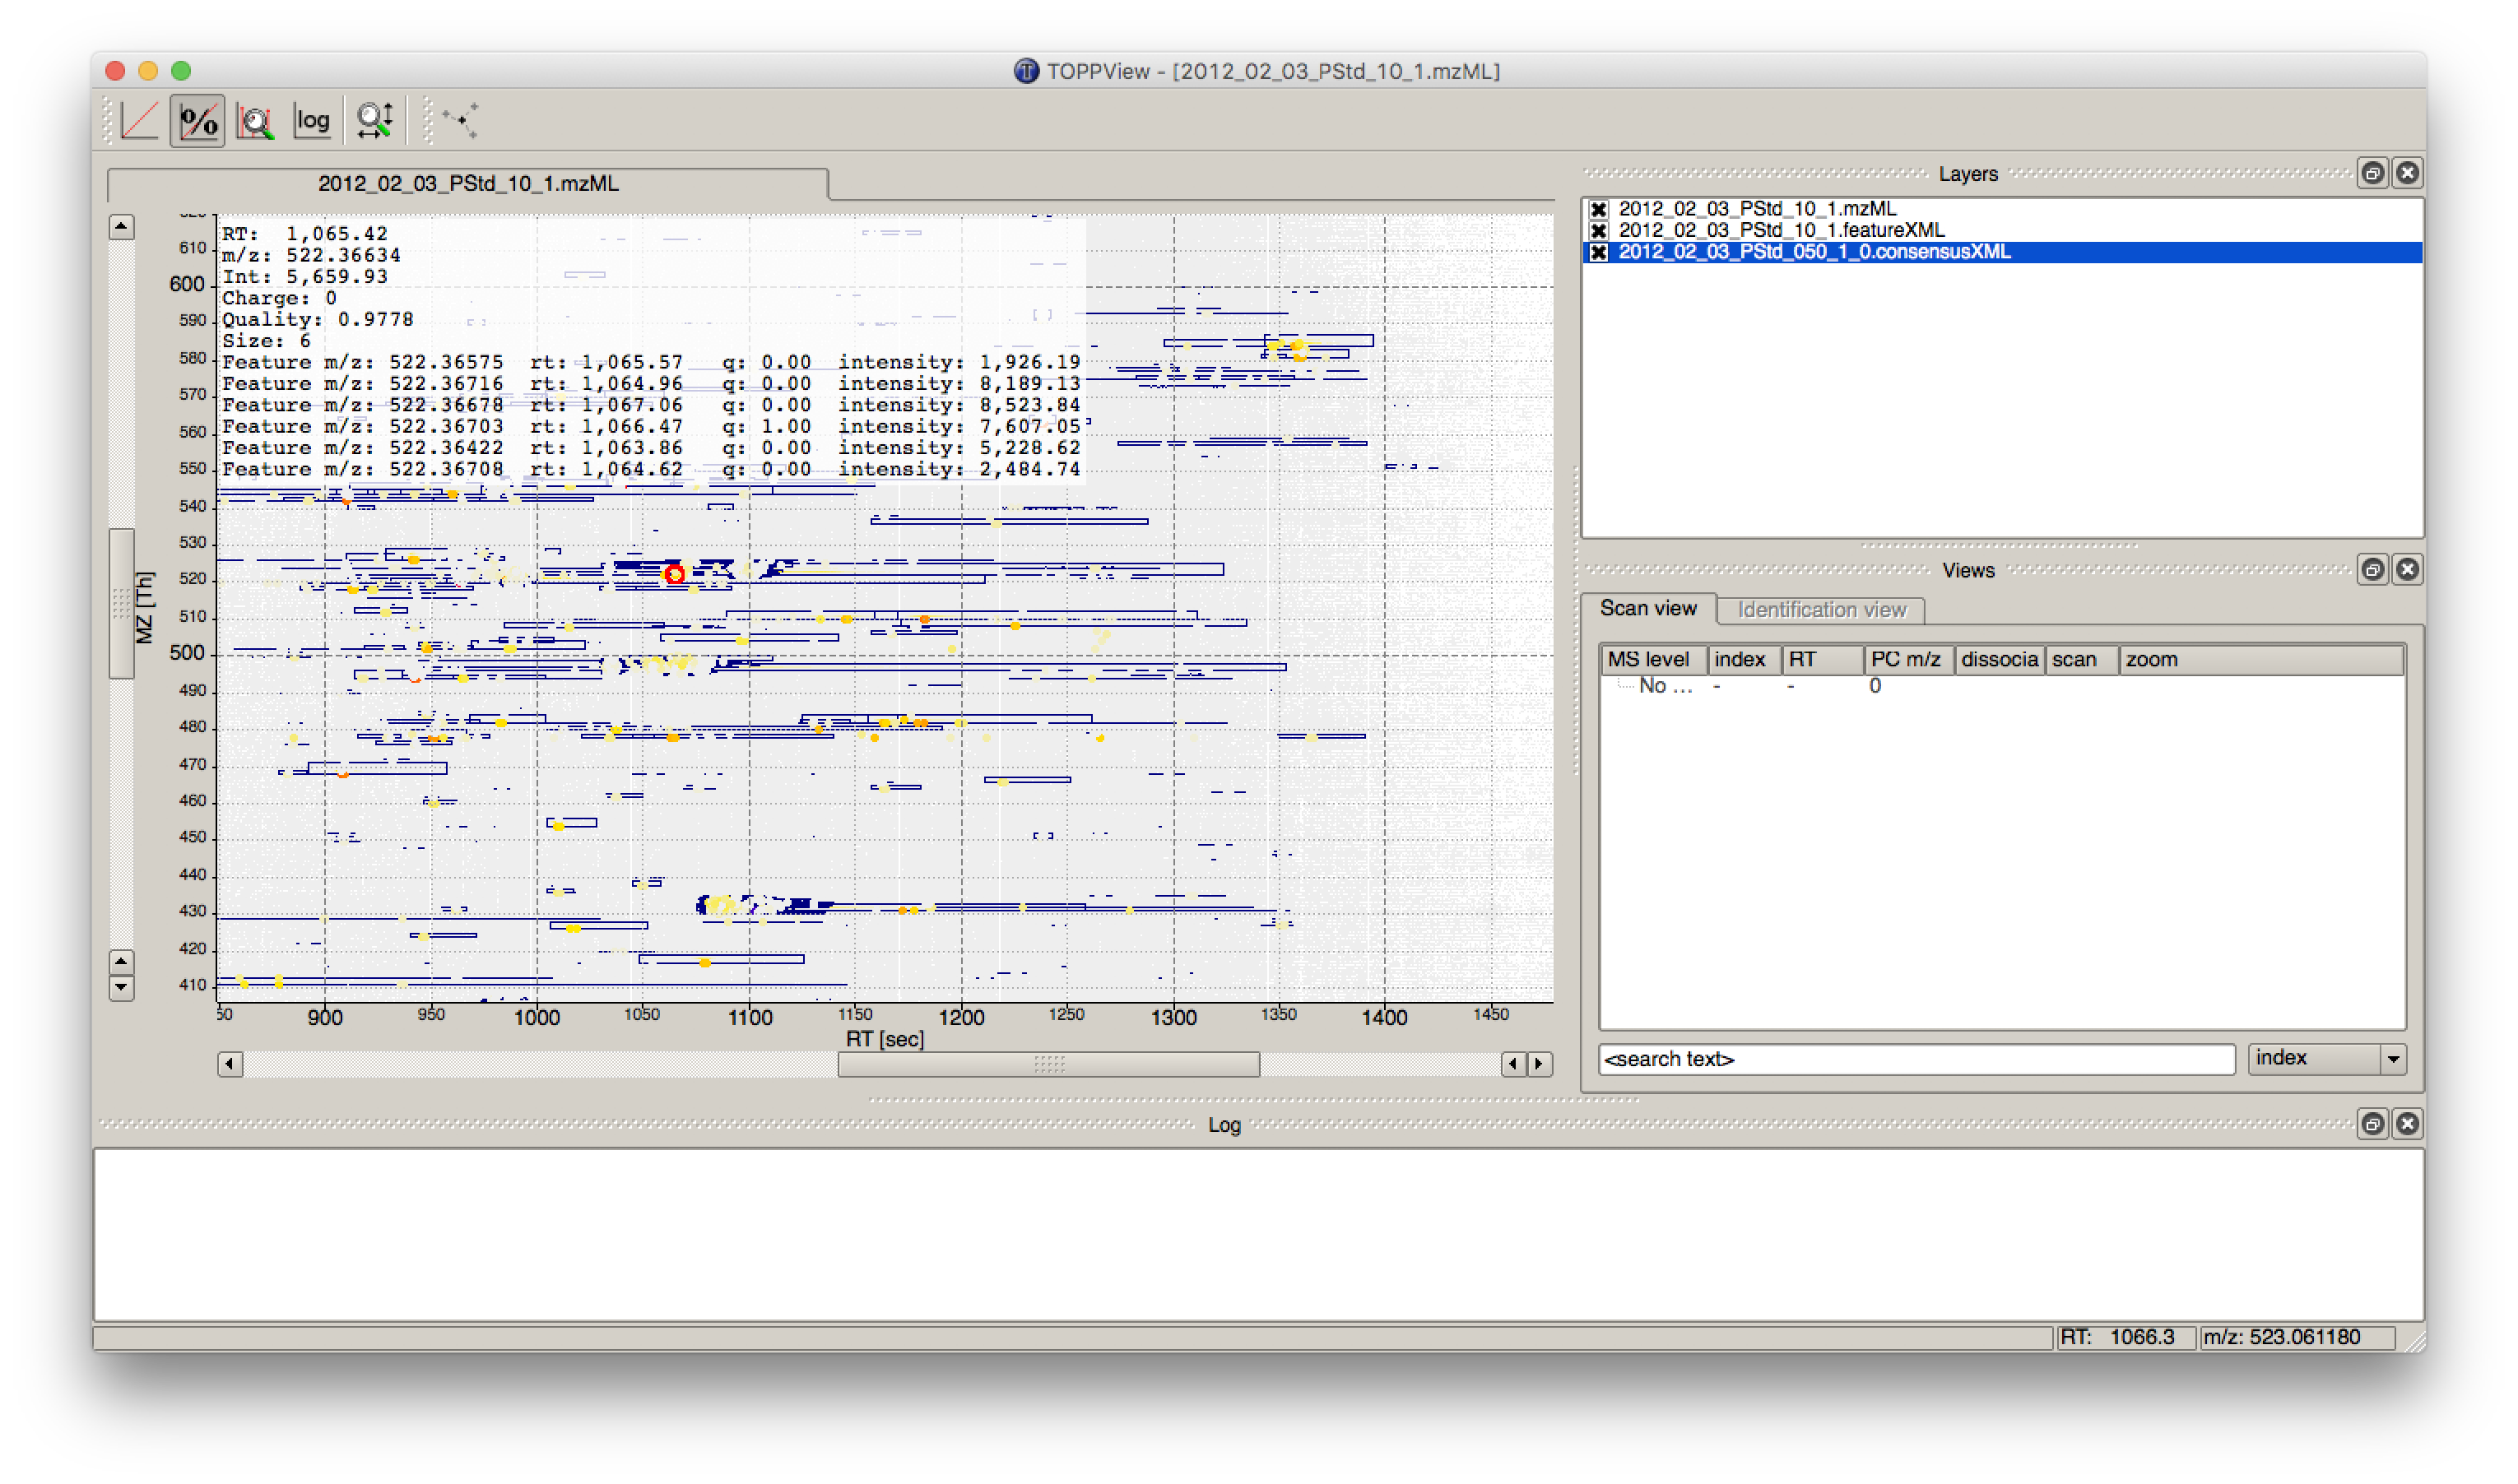
\includegraphics[width=\textwidth]{graphics/metabo/ToppView_5.png}
  \caption{Visualization of .consensusXML output over the .mzML and .featureXML 'layer'. }
  \label{fig:ToppView_5}
\end{figure}

\subsection{Basic metabolite identification}

At the current state we found several metabolites in the individual maps but so far don't know what they are.
To identify metabolites OpenMS provides multiple tools, including search by mass: the \KNIMENODE{AccurateMassSearch} node searches observed masses against the Human Metabolome Database (HMDB)\cite{Wishart2007,Wishart2009,Wishart2013}.
We start with the workflow from the previous section (see \cref{fig:metabo_part1}).

\begin{itemize}
\item
Add a \KNIMENODE{FileConverter} node (\menu{Community Nodes > OpenMS > File Handling}) and connect the output of the \KNIMENODE{FeatureLinkerUnlabeledQT} to the incoming port.
\item
Open the Configure dialog of the \KNIMENODE{FileConverter} and select the tab "OutputTypes".
In the drop down list for FileConverter.1.out select "featureXML".
\item
Add an \KNIMENODE{AccurateMassSearch} node (\menu{Community Nodes > OpenMS > Utilities}) and connect the output of the \KNIMENODE{FileConverter} to the first port of the \KNIMENODE{AccurateMassSearch}.
\item
Add four \KNIMENODE{Input File} nodes and configure them with the following files
\begin{itemize}
\item
\directory{Example\_Data / Metabolomics / databases / PositiveAdducts.tsv}\\
This file specifies the list of adducts that are considered in the positive mode. Each line contains the formula and charge of an adduct separated by a semicolon (e.g. M+H;1+). The mass of the adduct is calculated automatically.
\item
\directory{Example\_Data / Metabolomics / databases / NegativeAdducts.tsv}\\
This file specifies the list of adducts that are considered in the negative mode analogous to the positive mode.
\item
\directory{Example\_Data / Metabolomics / databases / HMDBMappingFile.tsv}\\
This file contains information from a metabolite database in this case from HMDB. It has three (or more) tab-separated columns: mass, formula, and identifier(s). This allows for an efficient search by mass.
\item
\directory{Example\_Data / Metabolomics / databases / HMDB2StructMapping.tsv}\\
This file contains additional information about the identifiers in the mapping file. It has four tab-separated columns that contain the identifier, name, SMILES, and INCHI. These will be included in the result file. The identifiers in this file must match the identifiers in the HMDBMappingFile.tsv.
\end{itemize}
\item
In the same order as they are given above connect them to the remaining input ports of the \KNIMENODE{AccurateMassSearch} node.
\item
Add an \KNIMENODE{Output Folder} node and connect the first output port of the \\
\KNIMENODE{AccurateMassSearch} node to the \KNIMENODE{Output Folder}.
\end{itemize}

The result of the \KNIMENODE{AccurateMassSearch} node is in the mzTab format \cite{Griss2014} so you can easily open it in a text editor or import it into Excel or KNIME, which we will do in the next section.
The complete workflow from this section is shown in \cref{fig:metabo_part2}.

\begin{figure}[htbp]
  \centering
  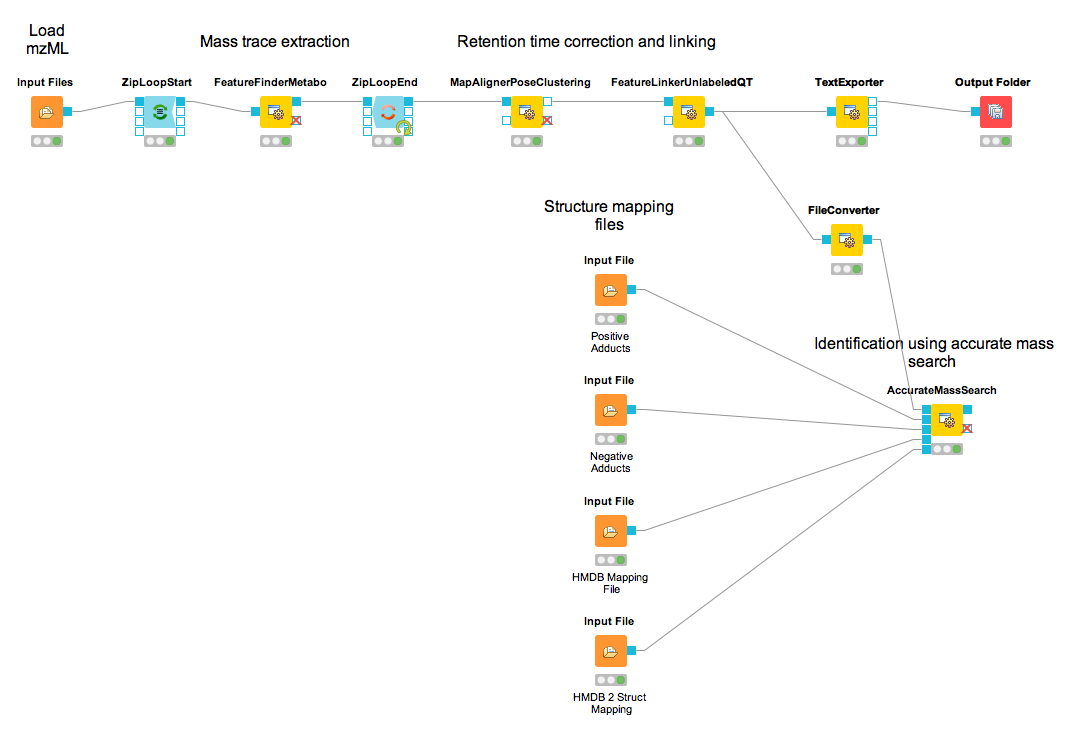
\includegraphics[width=0.85\textwidth]{graphics/metabo/metabo_part2.png}
  \caption{Label-free quantification and identification workflow for metabolites}
  \label{fig:metabo_part2}
\end{figure}

\subsubsection{Convert your data into a KNIME table}

The result from the \KNIMENODE{TextExporter} node as well as the result from the \KNIMENODE{AccurateMassSearch} node are files while standard KNIME nodes display and process only KNIME tables. To convert these files into KNIME tables we need two different nodes.
For the \KNIMENODE{AccurateMassSearch} results we use the \KNIMENODE{MzTabReader} node (\menu{Community Nodes > OpenMS > Conversion > mzTab}) and its \textit{Small Molecule Section} port. For the result of the \KNIMENODE{TextExporter} we use the \KNIMENODE{ConsensusTextReader} (\menu{Community Nodes > OpenMS > Conversion}).

When executed, both nodes will import the OpenMS files and provide access to the data as KNIME tables.
You can now easily combine both tables using the \KNIMENODE{Joiner} node (\menu{Manipulation > Column > Split \& Combine}) and configure it to match the m/z and retention time values of the respective tables.
The full workflow is shown in \cref{fig:metabo_part3}.

\begin{figure}[htbp]
  \centering
  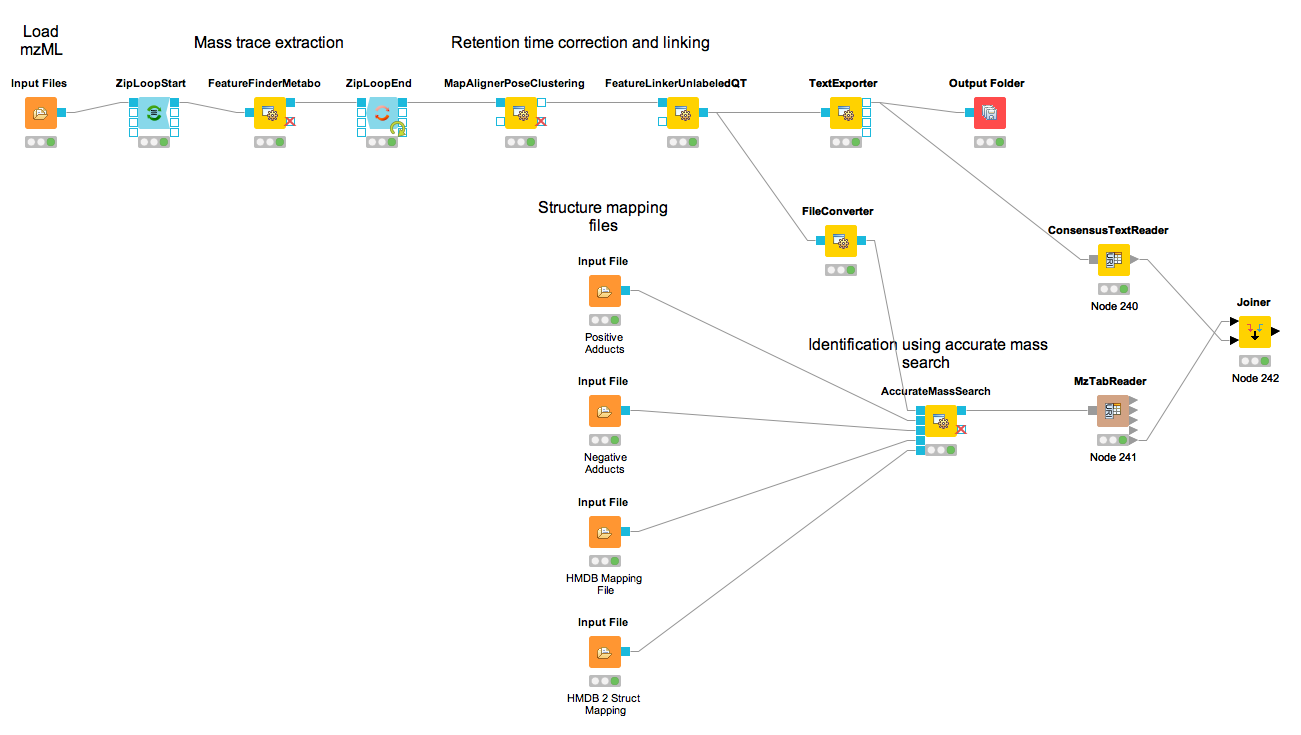
\includegraphics[width=0.85\textwidth]{graphics/metabo/metabo_part3.png}
  \caption{Label-free quantification and identification workflow for metabolites that loads the results into KNIME and joins the tables.}
  \label{fig:metabo_part3}
\end{figure}

\subsubsection{Visualizing data}

Now that you have your data in KNIME you should try to get a feeling for the capabilities of KNIME.

\begin{task}
Check out the \KNIMENODE{Molecule Type Cast}  node (\menu{Chemistry > Translators}) together with subsequent cheminformatics nodes (e.g. \KNIMENODE{RDKit From Molecule} (\menu{Community Nodes > RDKit > Converters})) to render the structural formula contained in the result table.

\end{task}
\begin{task}
Have a look at the \KNIMENODE{Column Filter} node to reduce the table to the interesting columns, e.g., only the Ids, chemical formula, and intensities.
\end{task}
\begin{task}
Try to compute and visualize the m/z and retention time error of the different feature elements (from the input maps) of each consensus feature. Hint: A nicely configured \KNIMENODE{Math Formula (Multi Column)} node should suffice.
\end{task}

\subsubsection{Spectral library search}

Identifying metabolites using only the accurate mass may lead to ambiguous results. In practice, additional information (e.g. the retention time) is used to further narrow down potential candidates. Apart from MS1-based features, tandem mass spectra (MS2) of metabolites provide additional information.
In this part of the tutorial, we take a look on how metabolite spectra can be identified using a library of previously identified spectra.

\noindent Because these libraries tend to be large we don't distribute them with OpenMS. 

\begin{task}
Construct the workflow as shown in Fig.~\ref{fig:speclib}.
Use the file \directory{Example\_Data / Metabolomics / datasets \newline / Metabolite\_ID\_SpectraDB\_positive.mzML} as input for your workflow.  You can use the spectral library from \\
\directory{Example\_Data / Metabolomics / databases / MetaboliteSpectralDB.mzML}\\ as second input. 
The first input file contains tandem spectra that are identified by the \KNIMENODE{MetaboliteSpectralMatcher}. The resulting mzTab file is read back into a KNIME table and stored in an Excel table. Make sure that you connect the MzTabReader port corresponding to the Small Molecule Section to the \KNIMENODE{Excel writer (XLS)}. Please select the "add column headers" option in the \KNIMENODE{Excel writer (XLS)}).

\end{task}

\begin{figure}[htbp]
  \centering
  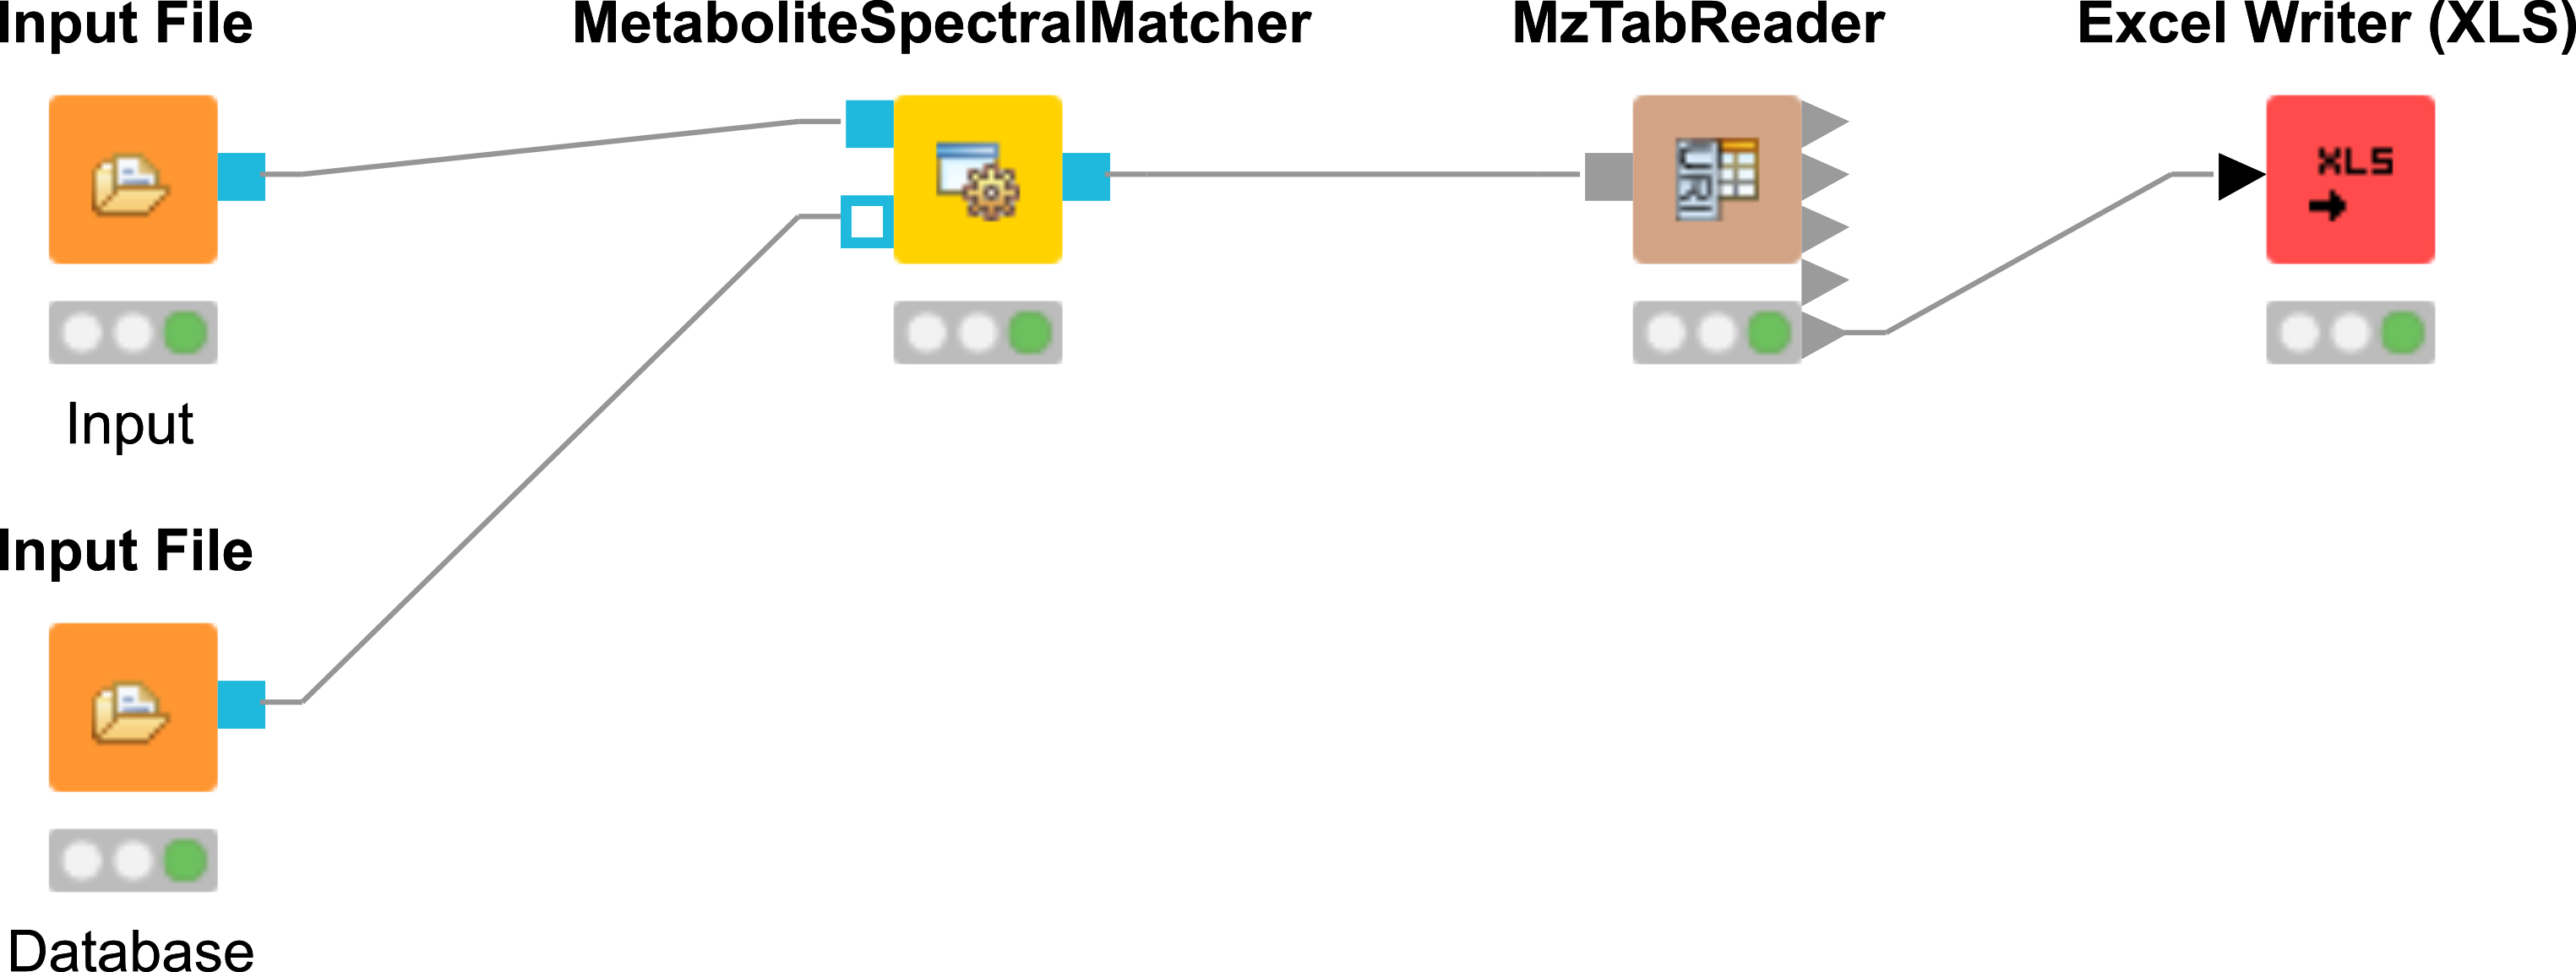
\includegraphics[width=0.7\textwidth]{graphics/metabo/speclib.png}
  \caption{Spectral library identification workflow}
  \label{fig:speclib}
\end{figure}

Run the workflow and inspect the output.

\subsubsection{Manual validation}

In metabolomics, matches between tandem spectra and spectral libraries are manually validated. Several commercial and free online resources exist which help in that task. Some examples are:

\begin{itemize}
\item mzCloud contains only spectra from Thermo Orbitrap instruments. The webpage requires Microsoft Silverlight which currently does not work in modern browsers (see \url{https://www.mzcloud.org/DataViewer}).
\item MassBank North America (MoNA) has spectra from different instruments but falls short in in number of spectra (compared to Metlin and mzCloud) \url{http://mona.fiehnlab.ucdavis.edu/spectra/display/KNA00122}
\item METLIN includes 961,829 molecules ranging from lipids, steroids, metabolites, small peptides, carbohydrates, exogenous drugs and toxicants. In total over 14,000 metabolites.
\end{itemize}

Here, we will use METLIN to manually validate metabolites.

\begin{task}
Check in the .xlsx output from the \KNIMENODE{Excel writer (XLS)} if you can find glutathione. Use the retention time column to find the spectrum in the mzML file. Here open the file in the \directory{Example\_Data / Metabolomics / datasets \newline / Metabolite\_ID\_SpectraDB\_positive.mzML} in  TOPPView. The MSMS spectrum with the retention time of 67.6 s is used as example. The spectrum can be selected based on the retention time in the scan view window. Therefore the MS1 spectrum with the retention time of 66.9 s has to be double clicked and the MSMS spectra recorded in this time frame will show up. Select the tandem spectrum of Glutathione, but do not close TOPPView, yet.
\end{task} 

\begin{figure}[htbp]
  \centering
  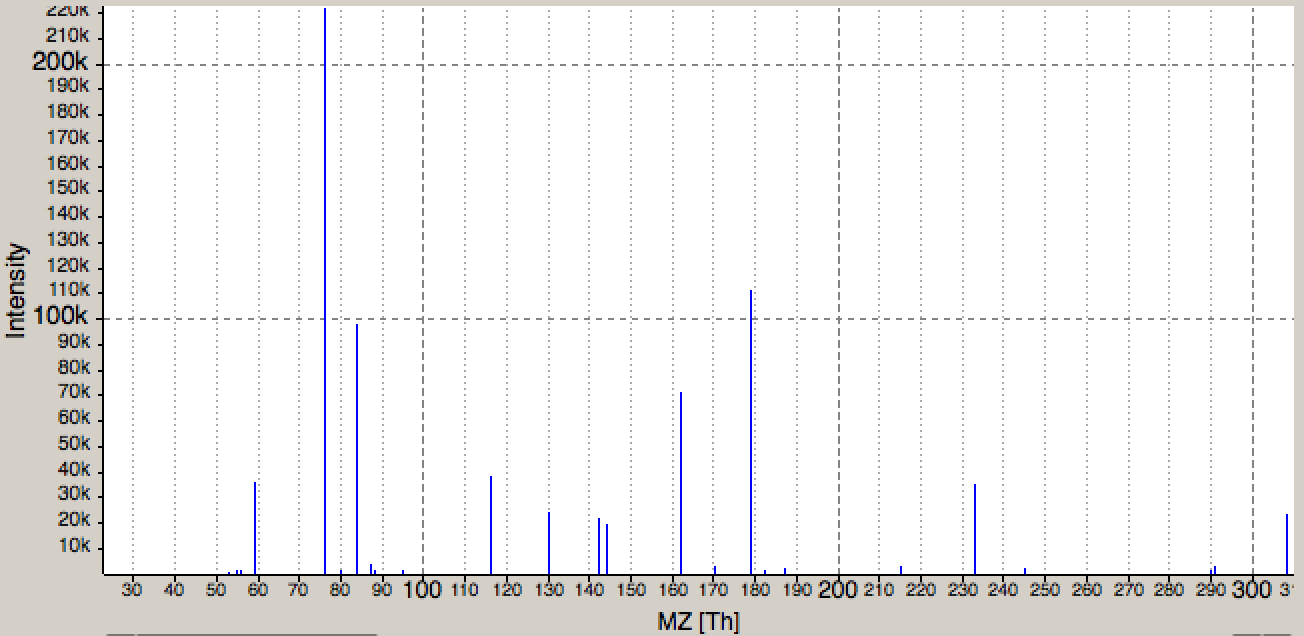
\includegraphics[width=0.85\textwidth]{graphics/metabo/glutathioneTV.png}
  \caption{Tandem spectrum of glutathione. Visualized in TOPPView.}
  \label{fig:glutathioneTandemSpectrum}
\end{figure}

\begin{task}
On the METLIN homepage search for \menu{Compound Name} Glutathione using the \menu{Advanced Search} (\url{https://metlin.scripps.edu/landing_page.php?pgcontent=advanced_search}). Note that free registration is required. Which collision energy (and polarity) gives the best (visual) match to your experimental spectrum in TOPPView? Here you can compare the fragmentation patterns in both spectra shown by the Intensity or relative Intensity, the m/z of a peak and the distance between peaks. Each distance between two peaks corresponds to a fragment of elemental composition (e.g., NH2 with the charge of one would have mass of two peaks of 16.023 Th).
\end{task}

\begin{figure}[htbp]
  \centering
  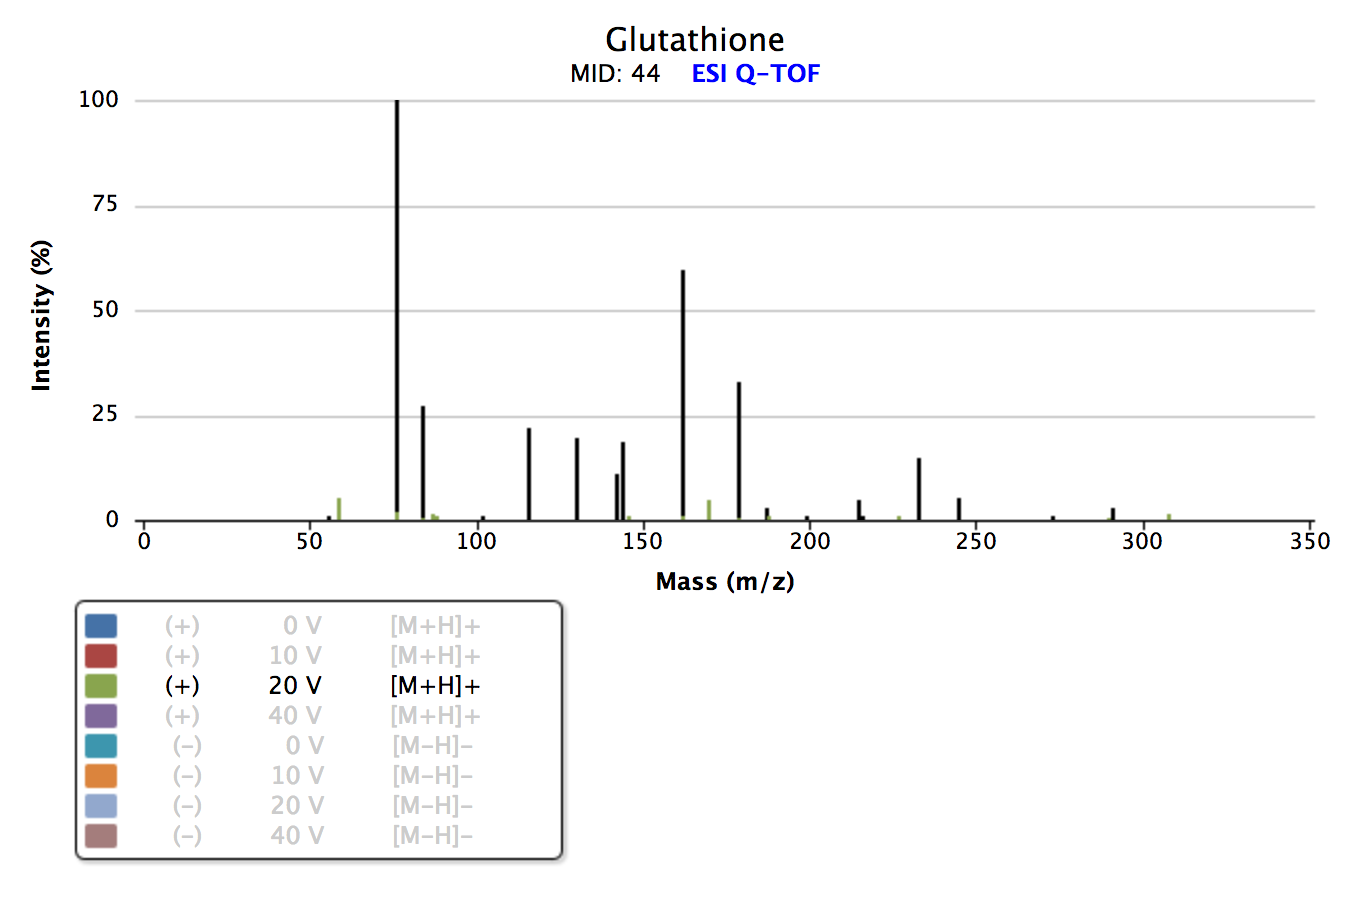
\includegraphics[width=0.85\textwidth]{graphics/metabo/glutathioneMetlin.png}
  \caption{Tandem spectrum of glutathione. Visualized in Metlin. Note that several fragment spectra from varying collision energies are available.}
  \label{fig:glutathioneMetlin}
\end{figure}

\subsubsection{De novo identification}

Another method for identification of metabolites using the MS2 spectra is de-novo identification. 
This can be used in addition to the other methods (accurate mass search, spectral library search) or individually if no spectral spectral library is available. In this part of the tutorial, we take a look on how metabolite spectra can be identified using de-novo tools. To this end, the tool SIRIUS and CSI:FingerID (\cite{Bocker2009,Bocker2016,Duhrkop2015}) was integrated in the OpenMS Framework as SiriusAdapter. SIRIUS uses isotope pattern analysis for detecting the molecular formula and further analyses the fragmentation pattern of a compound using fragmentation treesCSI:FingerID  is a method for searching a tandem mass spectrum of a small molecule (metabolite) in a database of molecular structures.

The is able to work in different modes depending on the provided input. 
\begin{itemize}
\item Input: mzML - SiriusAdapter will use the MS1 and MS2 information provided and search all MS2 spectra in a map.  
\item Input: mzML, featureXML (FeatureFinderMetabo) - SiriusAdapter can use the provided feature information to reduce the search space to valid Features with MS2 spectra. Additional it can use the Isotope trace information. 
\item Input: mzML, featureXML (FeatureFinderMetabo and MetaboliteAdductDecharger) - SiriusAdapter can use the feature information as mentioned above. Further adduct information of the feature is provided by using adduct grouping. 
\end{itemize}

The last method is the preferred one, since SIRIUS gains a lot of additional information by using the OpenMS preprocessing. 

\begin{task}
Construct the workflow as shown in Fig.~\ref{fig:denovoid}. \\
Use the file \directory{Example\_Data / Metabolomics / datasets \newline / Metabolite\_DeNovoID\.mzML} as input for your workflow.  
\end{task}

\begin{figure}[htbp]
  \centering
  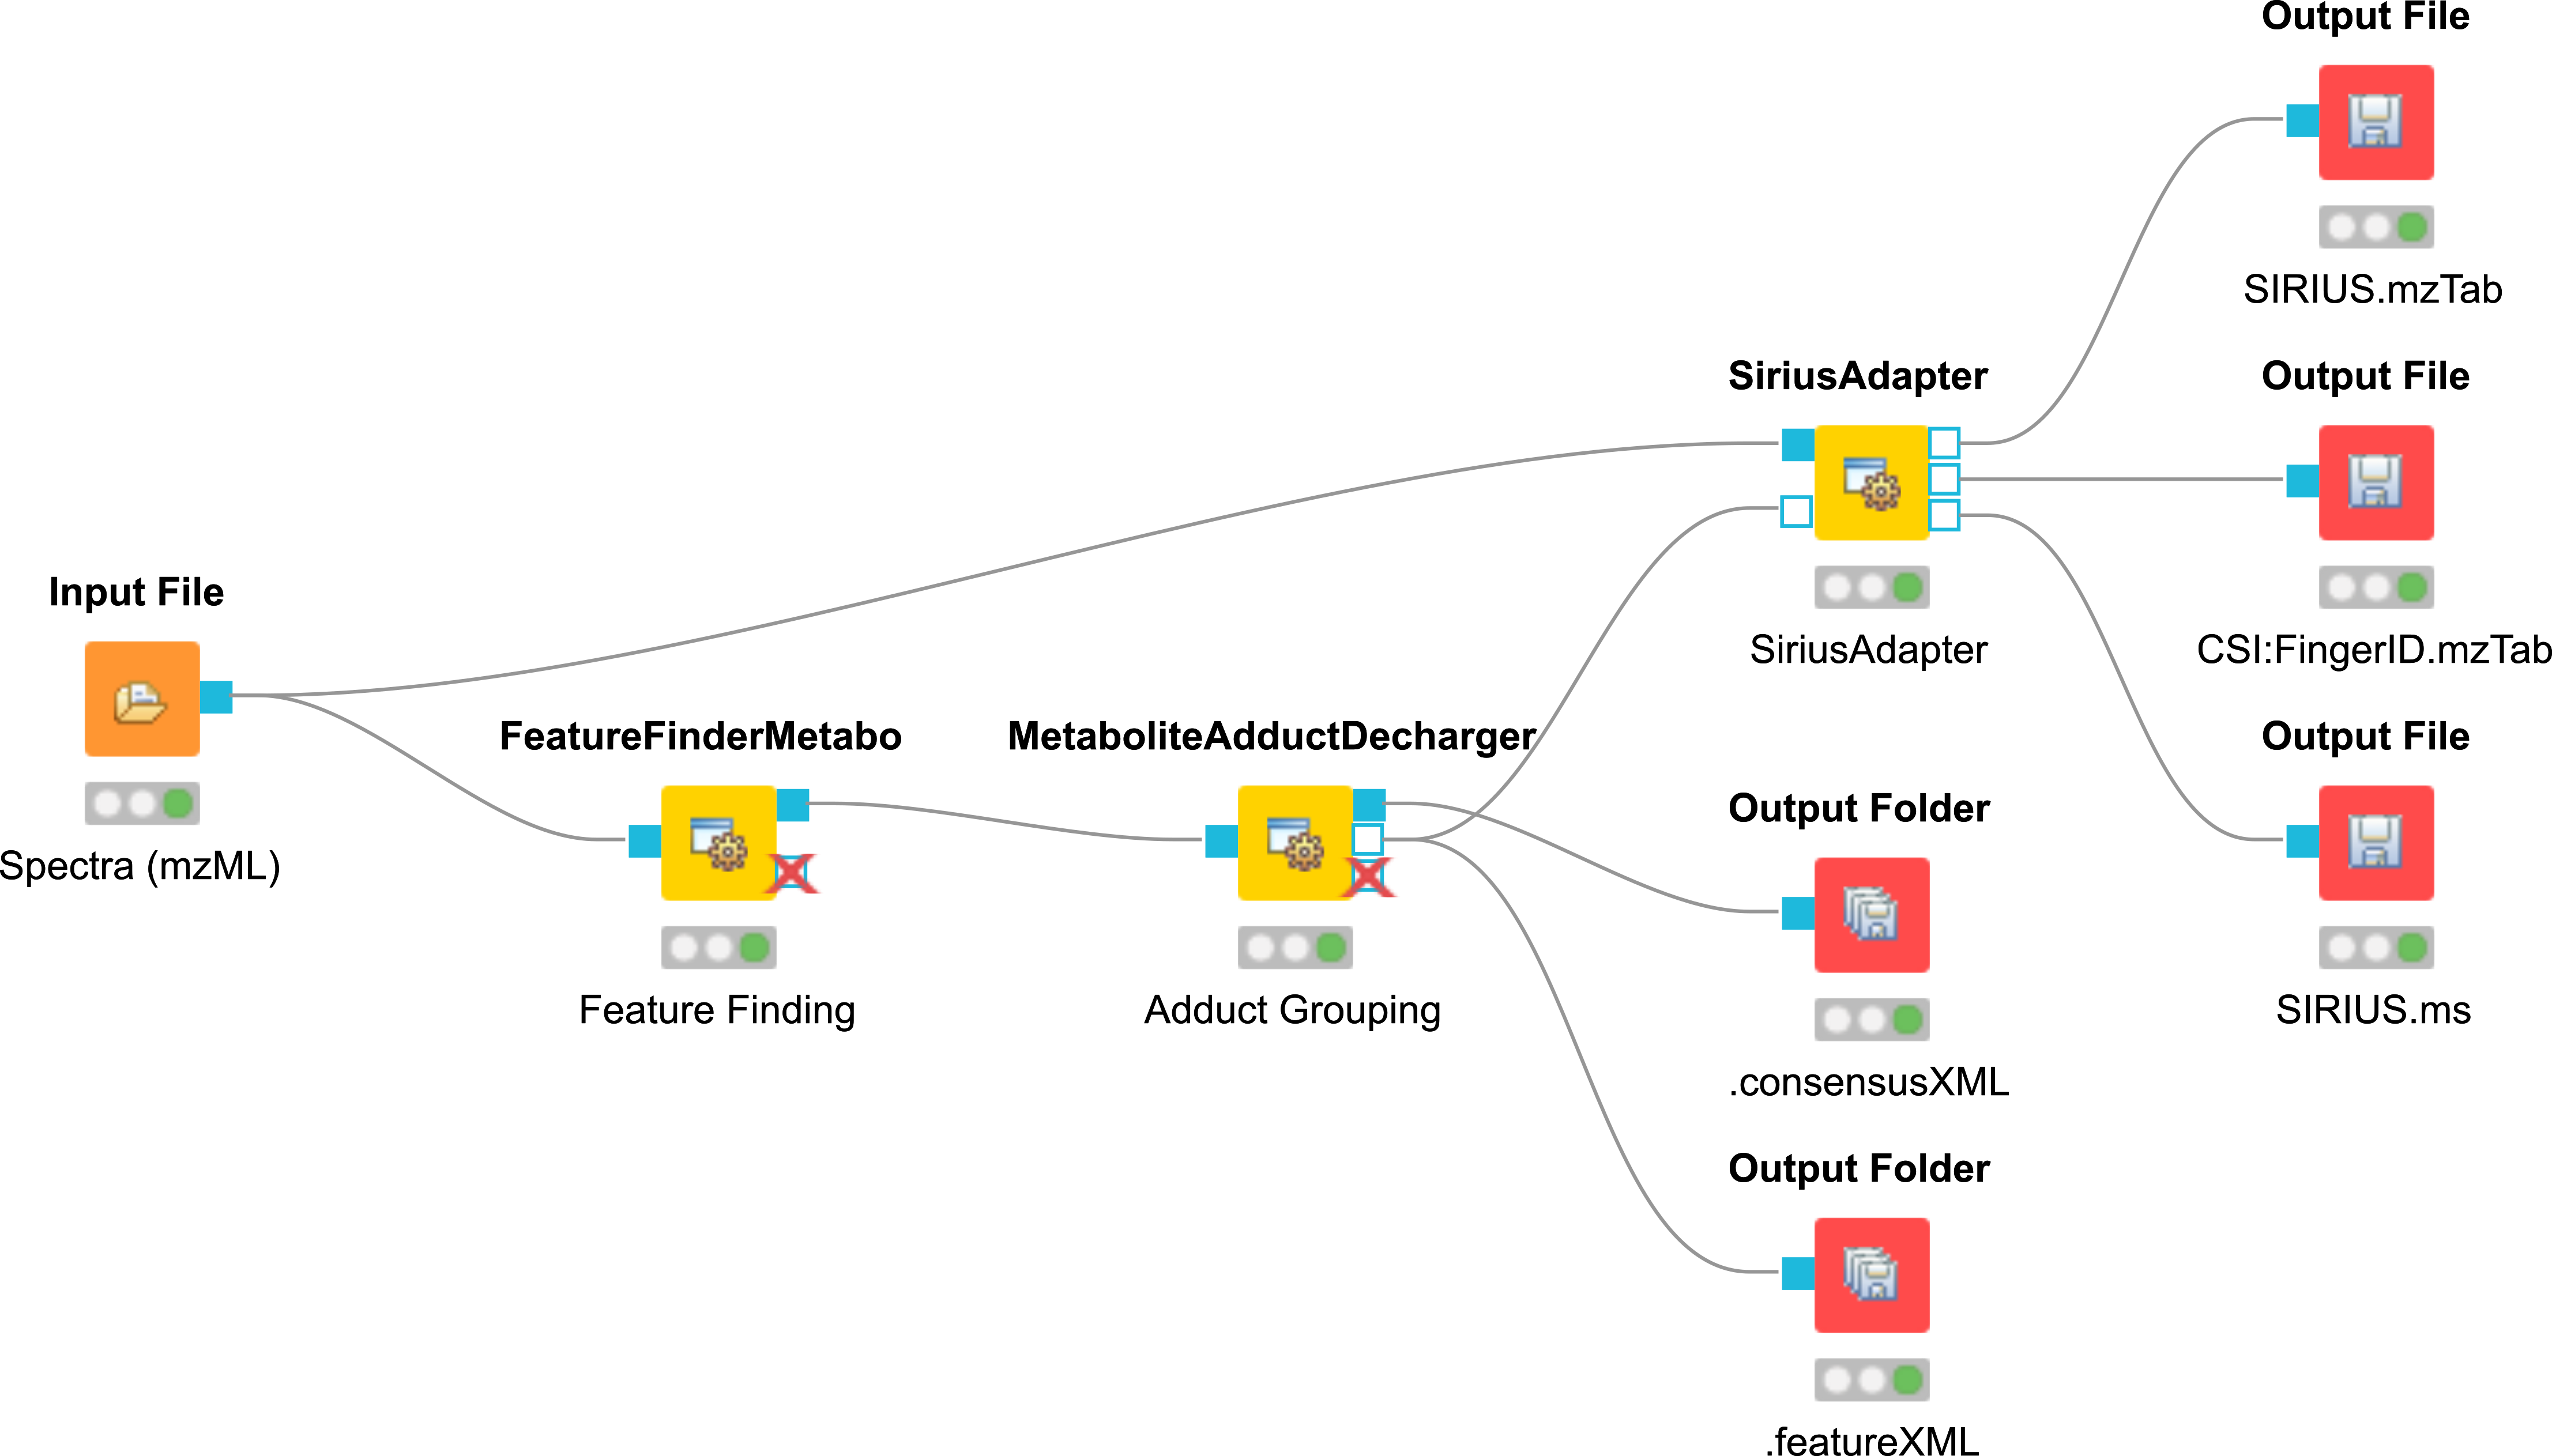
\includegraphics[width=0.85\textwidth]{graphics/metabo/denovoid.png}
  \caption{De novo identification workflow}
  \label{fig:denovoid}
\end{figure}

Run the workflow and inspect the output. \\

\noindent The output consists of two mzTab files . One for the SIRIUS and the other for the CSI:FingerID summary. These provide information about the sumformula, adduct and the possible compound structure. The information is referenced to the spectrum used in the analysis. Additional information can be extracted by using the \KNIMENODE{SiriusAdapter} debug output. Here the SIRIUS workspace will be provided after the calculation has finished. The folder contains information about annotated fragments for each successfully explained compound.  

The debug folder can be found by selecting the \KNIMENODE{SiriusAdapter} after the workflow has finished and using its \menu{View: SiriusAdapter Std Output}. Here the path found in \menu{Keeping temporary files in directory}can be copied to your file manger - this will be simplified in the next OpenMS release.

%%%%%%%%%%%%%%%%%%%%%%%%%%%%%%%%%%%%%%%%%%%%%%%%%%%%%%%%%%%%%%%%%%%%%%%%%%%%%%%%%%%%%%%%%%%%%%%%%%%%%%%%%%%%%%%%%%%%%%%%%%%%%%%%%%%%
\subsection{Downstream data analysis and reporting}
In this part of the metabolomics session we take a look at more advanced downstream analysis and the use of the statistical programming language R. As laid out in the introduction we try to detect a set of spike-in compounds against a complex blood background. As there are many ways to perform this type of analysis we provide a complete workflow.

\begin{task}
Import the workflow from \directory{Workflows / metabolite\_ID.knwf} in KNIME: \menu{File > Import KNIME Workflow...}
\end{task}

The section below will guide you in your understanding of the different parts of the workflow. Once you understood the workflow you should play around and be creative. Maybe create a novel visualization in KNIME or R? Do some more elaborate statistical analysis? Note that some basic R knowledge is required to fully understand the processing in \KNIMENODE{R Snippet} nodes.

\subsubsection{Signal processing and data preparation for identification}
This part is analogous to what you did for the simple metabolomics pipeline.

\subsubsection{Data preparation for quantification}
The first part is identical to what you did for the simple metabolomics pipeline. Additionally, we convert zero intensities into NA values and remove all rows that contain at least one NA value from the analysis. We do this using a very simple \KNIMENODE{R Snippet} and subsequent \KNIMENODE{Missing Value filter} node.

\begin{task}
Inspect the \KNIMENODE{R Snippet} by double-clicking on it. The KNIME table that is passed to an \KNIMENODE{R Snippet} node is available in R as a data.frame named knime.in. The result of this node will be read from the data.frame knime.out after the script finishes. Try to understand and evaluate parts of the script (Eval Selection). In this dialog you can also print intermediary results using for example the R command head(knime.in) or cat(knime.in) to the Console pane.
\end{task}

\subsubsection{Statistical analysis}
After we linked features across all maps, we want to identify features that are significantly deregulated between the two conditions. We will first scale and normalize the data, then perform a t-test, and finally correct the obtained p-values for multiple testing using Benjamini-Hochberg. All of these steps will be carried out in individual \KNIMENODE{R Snippet} nodes.
\begin{itemize}
\item Double-click on the first \KNIMENODE{R Snippet} node labeled "log scaling" to open the \KNIMENODE{R Snippet} dialog. In the middle you will see a short R script that performs the log scaling. To perform the log scaling we use a so-called regular expression (grepl) to select all columns containing the intensities in the six maps and take the $log_2$ logarithm.

\item The output of the log scaling node is also used to draw a boxplot that can be used to examine the structure of the data. Since we only want to plot the intensities in the different maps (and not m/z or rt) we first use a \KNIMENODE{Column Filter} node to keep only the columns that contain the intensities. We connect the resulting table to a \KNIMENODE{Box Plot} node which draws one box for every column in the input table. Right-click and select \menu{View: Box Plot}.

\item The median normalization is performed in a similar way to the log scaling. First we calculate the median intensity for each intensity column, then we subtract the median from every intensity.

\item Open the \KNIMENODE{Box Plot} connected to the normalization node and compare it to the box plot connected to the log scaling node to examine the effect of the median normalization.

\item To perform the t-test we defined the two groups we want to compare. Then we call the t-test for every consensus feature unless it has missing values. Finally we save the p-values and fold-changes in two new columns named p-value and FC.

\item The \KNIMENODE{Numeric Row Splitter} is used to filter less interesting parts of the data. In this case we only keep columns where the fold-change is $\geq$ 2.

\item We adjust the p-values for multiple testing using Benjamini-Hochberg and keep all consensus features with a q-value $\leq$ 0.01 (i.e. we target a false-discovery rate of $1\%$).

\end{itemize}


\subsubsection{Interactive visualization}

KNIME supports multiple nodes for interactive visualization with interrelated output. The nodes used in this part of the workflow exemplify this concept. They further demonstrate how 
figures with data dependent customization can be easily realized using basic KNIME nodes. Several simple operations are concatenated in order to enable an interactive volcano plot.
\begin{itemize}
\item We first log-transform fold changes and p-values in the \KNIMENODE{R Snippet} node. We then append columns noting interesting features (concerning fold change and p-value).
\item With this information, we can use various Manager nodes (\menu{Views > Property}) to emphasize interesting data points. The configuration dialogs allow us to select columns to change color, shape or size of data points dependent on the column values.
\item The \KNIMENODE{Scatter Plot} node (\menu{Views}) enables interactive visualization of the logarithmized values as a volcano plot: the log-transformed values can be chosen in the `Column Selection' tab of the plot view. Data points can be selected in the plot and HiLited via the menu option. HiLiteing transfers to all other interactive nodes connected to the same data table. In our case, selection and HiLiteing will also occur in the \KNIMENODE{Interactive Table} node (\menu{Views}).
\item Output of the interactive table can then be filtered via the HiLite menu tab. For example, we could restrict shown rows to points HiLited in the volcano plot.
\end{itemize}
\begin{task}
Inspect the nodes of this section. Customize your visualization and possibly try to visualize other aspects of your data.
\end{task}

\subsubsection{Advanced visualization}
\label{sec:metaboR}
R Dependencies: This section requires that the R packages \texttt{ggplot2} and \texttt{ggfortify} are both installed. \texttt{ggplot2} is part of the \textit{KNIME R Statistics Integration (Windows Binaries)} which should already be installed via the full KNIME installer, \texttt{ggfortify} however is not.
In case that you use an R installation where one or both of them are not yet installed, add an \KNIMENODE{R Snippet} node and double-click to configure. In the \textit{R Script} text editor, enter the following code:
\begin{lstlisting}
#Include the next line if you also have to install ggplot2:
install.packages("ggplot2")
#Include the following lines to install ggfortify:
install.packages("ggfortify")
library(ggplot2)
library(ggfortify)
\end{lstlisting}
You can remove the \texttt{install.packages} commands once it was successfully installed.

Even though the basic capabilities for (interactive) plots in KNIME are valuable for initial data exploration, professional looking depiction of analysis results often relies on dedicated plotting libraries. The statistics language R supports the addition of a large variety of packages, including packages providing extensive plotting capabilities. This part of the workflow shows how to use R nodes in KNIME to visualize more advanced figures. Specifically, we make use of different plotting packages to realize heatmaps.


\begin{itemize}
\item The used \KNIMENODE{RView (Table)} nodes combine the possibility to write R snippet code with visualization capabilities inside KNIME. Resulting images can be looked at in the output RView, or saved via the \KNIMENODE{Image Port Writer} node.
\item The heatmap nodes make use of the gplots libary, which is by default part of the R Windows binaries (for full KNIME version 3.1.1 or higher). We again use regular expressions to extract all measured intensity columns for plotting. For clarity, feature names are only shown in the heatmap after filtering by fold changes.
\end{itemize}

\subsubsection{Data preparation for Reporting}
Following the identification, quantification and statistical analysis our data is merged and formatted for reporting.
First we want to discard our normalized and logarithmized intensity values in favor of the original ones.
To this end we first remove the intensity columns (\KNIMENODE{Column Filter}) and add the original intensities back (\KNIMENODE{Joiner}).
For that we use an \textit{Inner Join} \footnote{\textit{Inner Join} is a technical term that describes how database tables are merged.} with the \KNIMENODE{Joiner} node. In the dialog of the node we add two entries for the Joining Columns and for the first column we pick "retention\_time" from the top input (i.e. the AccurateMassSearch output) and "rt\_cf" (the retention time of the consensus features) for the bottom input (the result from the quantification). For the second column you should choose "exp\_mass\_to\_charge" and "mz\_cf" respectively to make the joining unique. Note that the workflow needs to be executed up to the previous nodes for the possible selections of columns to appear.

\begin{figure}[htbp]
  \centering
  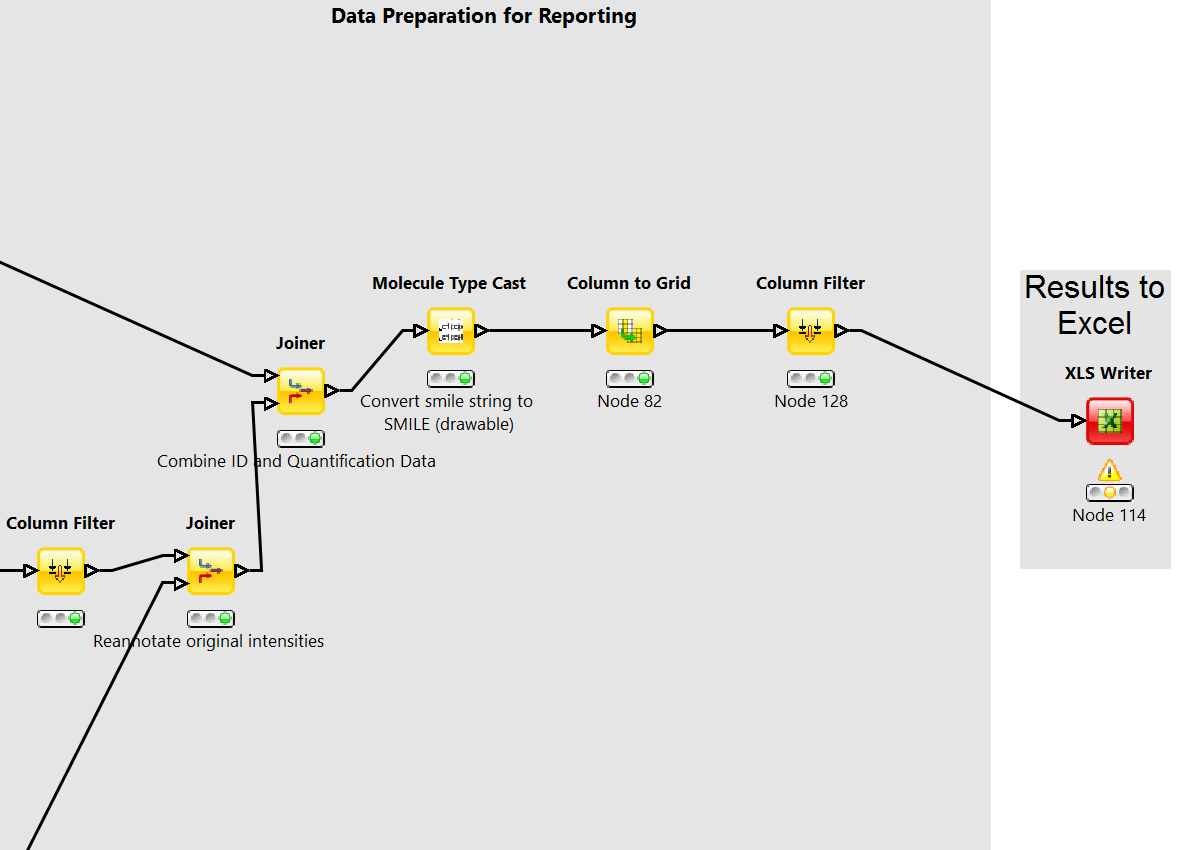
\includegraphics[width=0.7\textwidth]{graphics/metabo/reporting.png}
  \caption{Data preparation for reporting}
  \label{fig:reporting}
\end{figure}

\begin{question}
What happens if we use a \textit{Left Outer Join}, \textit{Right Outer Join} or \textit{Full Outer Join} instead of the \textit{Inner Join}?
\end{question}

\begin{task}
Inspect the output of the join operation after the Molecule Type Cast and RDKit molecular structure generation.
\end{task}

While all relevant information is now contained in our table the presentation could be improved.
Currently, we have several rows corresponding to a single consensus feature (=linked feature) but with different, alternative identifications.
It would be more convenient to have only one row for each consensus feature with all accurate mass identifications added as additional columns.
To this end, we use the \KNIMENODE{Column to Grid} node that flattens several rows with the same consensus number into a single one.
Note that we have to specify the maximum number of columns in the grid so we set this to a large value (e.g. 100).
We finally export the data to an Excel file (\KNIMENODE{XLS Writer}).




%%%%%%%%%%%%%%%%%%%%%%%%%%%%%%%%%%%%%%%%%%%%%%%%%%%%%%%%%%%%%%%%%%%%%%%%%%%
%\newpage

\bibliographystyle{phreporturl}
\bibliography{handout}

\end{document}
